\chapter{Maximal extension of Schwarzschild spacetime}
\label{s:max}

\minitoc

\section{Introduction}


%%%%%%%%%%%%%%%%%%%%%%%%%%%%%%%%%%%%%%%%%%%%%%%%%%%%%%%%%%%%%%%%%%%%%%%%%%%%%%%


\section{Kruskal-Szekeres coordinates}

\subsection{Definition} \label{s:sch:KS_coord}

On the open set $\M_{\rm I}$, let us consider the ``double-null''
coordinate system $\hat{\hat{x}}^\alpha = (u,v,\th,\ph)$. It is related to
Schwarzschild-Droste coordinates $(t,r,\th,\ph)$ by
Eqs.~(\ref{e:sch:outgoing_null_geod})-(\ref{e:sch:ingoing_null_geod}):
\be \label{e:sch:u_v_r_t}
    \left\{\begin{array}{l}
    u = t - r - 2 m \ln \left| \frac{r}{2m} - 1 \right| \\[1ex]
    v = t + r + 2 m \ln \left| \frac{r}{2m} - 1 \right|
    \end{array}\right.
    \iff
        \left\{\begin{array}{l}
    t = \frac{1}{2} (u+v)\\[1ex]
    r + 2 m \ln \left| \frac{r}{2m} - 1 \right| = \frac{1}{2} (v-u).
    \end{array}\right.
\ee
Despite one cannot express explicitely $r$ in terms of $(u,v)$,
the function $r\mapsto r + 2 m \ln \left| \frac{r}{2m} - 1 \right|$ is
invertible on $(2m,+\infty)$ (cf. Fig.~\ref{f:sch:tortoise}), so that (\ref{e:sch:u_v_r_t}) does define a coordinate system on $\M_{\rm I}$.
The range of $(u,v)$ is $\R^2$.

The above relations imply
\[
 \D u = \D t - \frac{\D r}{1 - \frac{2m}{r}}  \qquad\mbox{and}\qquad
\D v = \D t + \frac{\D r}{1 - \frac{2m}{r}} .
\]
Hence
\[
    \D u \, \D v = \D t^2 - \frac{\D r^2}{\left(1 - \frac{2m}{r} \right) ^2} .
\]
The line element (\ref{e:sch:Schwarz_metric_SD}) becomes then
\be \label{e:sch:Schwarz_metric_uv}
    \encadre{
        \hat{\hat{g}}_{\mu\nu}\, \D \hat{\hat{x}}^\mu \,
        \D \hat{\hat{x}}^\nu =
            -\left( 1 - \frac{2 m}{r} \right)\, \D u \, \D v
       +  r^2 \left( \D\th^2 + \sin^2\th\, \D\ph^2 \right) }.
\ee
In this formula, $r$ is to be considered as a function of $(u,v)$, given
by (\ref{e:sch:u_v_r_t}).

\begin{figure}
\centerline{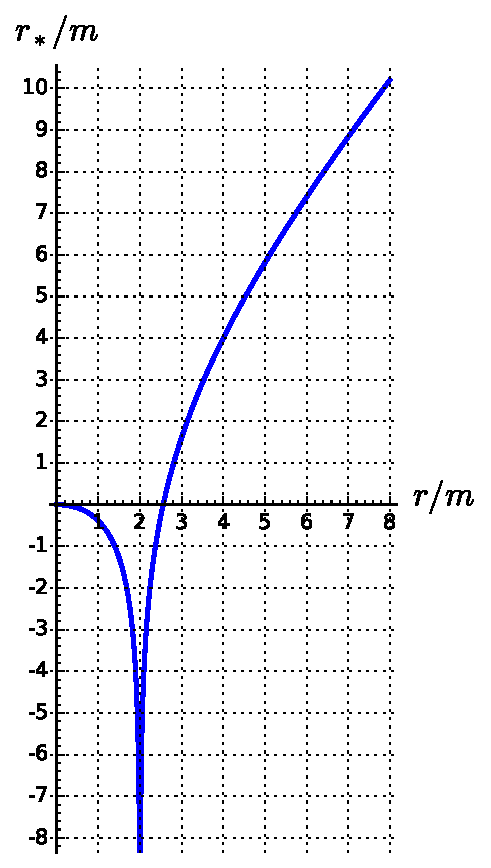
\includegraphics[height=0.4\textheight]{sch_tortoise.pdf}}
\caption[]{\label{f:sch:tortoise} \footnotesize
Function $r_*(r) = r + 2 m \ln \left| \frac{r}{2m} - 1 \right|$
(the tortoise coordinate, cf. Eq.~(\ref{e:sch:def_tortoise})).
It relates $r$ to $(u,v)$ via $r_*(r) = (u-v)/2$ [Eq.~(\ref{e:sch:u_v_r_t})].}
\end{figure}

The metric components (\ref{e:sch:Schwarz_metric_uv}) are regular on $\M_{\rm I}$.
Having a look at Fig.~\ref{f:sch:tortoise}, we realize that we cannot extend
this coordinate system to include the Schwarzschild horizon $\Hor$, since
$r\rightarrow 2m$ is equivalent to $v-u\rightarrow -\infty$: if $u$ (resp. $v$)
were taking a finite value on $\Hor$, we would have $v\rightarrow -\infty$
(resp. $u\rightarrow +\infty$). This impossibility of extending to $\Hor$
is also reflected by the fact that
\[
    \det \left( \hat{\hat{g}}_{\alpha\beta} \right) =
        - \frac{1}{4} \left( 1 - \frac{2 m}{r} \right) ^2 r^4 \sin^2\th
\]
vanishes for $r\rightarrow 2m$, which would make $\w{g}$ a degenerate bilinear
form at $r=2m$, while it is not of course.

Instead of $(u,v)$, let us use on $\M_{\rm I}$
the coordinates $(U,V)$ defined by
\be \label{e:sch:def_U_V}
    \left\{\begin{array}{l}
    U := - \mathrm{e}^{-u/4m} \\
    V := \mathrm{e}^{v/4m} .
    \end{array}\right.
\ee
Since the range of $(u,v)$ is $\R^2$, the range of $U$ is $(-\infty,0)$
and that of $V$ is $(0,+\infty)$.
We have
\[
    \D U = \frac{1}{4m} \,  \mathrm{e}^{-u/4m}  \, \D u\qquad\mbox{and}\qquad
    \D V = \frac{1}{4m} \,  \mathrm{e}^{v/4m} \, \D v ,
\]
hence
\[
    \D u \, \D v = 16 m^2 \mathrm{e}^{(u-v)/4m} \, \D U \, \D V .
\]
Now, on $\M_{\rm I}$, $r>2m$ and (\ref{e:sch:u_v_r_t}) yields
\be \label{e:sch:r_u_v_exp}
    r + 2 m \ln \left( \frac{r}{2m} - 1 \right) = \frac{1}{2} (v-u)
    \quad
    \Longrightarrow
    \quad
     \mathrm{e}^{r/2m} \left( \frac{r}{2m} - 1 \right)  =
    \mathrm{e}^{(v-u)/4m}  ,
\ee
so that
\[
     \D u \, \D v = 16 m^2 \, \mathrm{e}^{-r/2m}
        \left( \frac{r}{2m} - 1 \right) ^{-1} \D U \, \D V
        = \frac{32 m^3}{r} \, \mathrm{e}^{-r/2m}
        \left( 1 - \frac{2m}{r} \right) ^{-1} \D U \, \D V .
\]
Substituting this expression in (\ref{e:sch:Schwarz_metric_uv}) yields
the expression of the metric components with respect to
coordinates ${\hat X}^\alpha := (U,V,\th,\ph)$:
\be \label{e:sch:metric_UV}
    \encadre{
    g_{\mu\nu} \, \D {\hat X}^\mu \, \D {\hat X}^\nu =
    - \frac{32 m^3}{r} \, \mathrm{e}^{-r/2m} \,  \D U \, \D V
     +  r^2 \left( \D\th^2 + \sin^2\th\, \D\ph^2 \right) }.
\ee
In this formula, $r$ has to be considered as a function of $(U,V)$, whose
implicit expression is found by combining
(\ref{e:sch:def_U_V}) and (\ref{e:sch:r_u_v_exp}):
\be \label{e:max:r_UV_M_I}
    \encadre{ \mathrm{e}^{r/2m} \left( \frac{r}{2m} - 1 \right) = - U V } .
\ee
\begin{remark}
This relation takes a very simple form in terms of the tortoise coordinate
(cf. Eq.~(\ref{e:sch:def_tortoise})):
\be
    \mathrm{e}^{r_*/2m} = - U V  .
\ee
\end{remark}

We notice that the factor $(1-2m/r)$ has disappeared in the line
element (\ref{e:sch:metric_UV}), which becomes perfectly regular as
$r\rightarrow 2m$.

We read on (\ref{e:sch:metric_UV}) that $g_{UU} = 0$ and $g_{VV} = 0$.
Hence $(U,V)$ is a double-null coordinate system, as much as $(u,v)$.
To cope with a timelike-spacelike coordinate system instead, let
us introduce on $\M_{\rm I}$ the pair $(T,X)$ such that $U$ is $T$
retarded by $X$ and $V$ is $T$ advanced by $X$:
\be \label{e:sch:def_T_X}
    \left\{\begin{array}{l}
    U = T - X\\
    V = T + X
    \end{array}\right.
    \qquad \iff\qquad
    \left\{\begin{array}{l}
    T = \frac{1}{2} (U+V) \\[1ex]
    X = \frac{1}{2} (V-U)
    \end{array}\right.
\ee
Since the range of $U$ on $\M_{\rm I}$ is $(-\infty,0)$ and that of $V$ is
$(0,+\infty)$, the range of $(T,X)$ is ruled by $T<X$, $T>-X$ and $X>0$.
In other words, the coordinates $(T,X)$ span the following quarter of
$\mathbb{R}^2$ (cf. Fig.~\ref{f:sch:SD_I_KS}):
\be \label{e:sch:X_T_range_I}
    \M_{\rm I}: \quad X > 0 \quad\mbox{and}\quad -X < T < X .
\ee
The coordinates $X^\alpha := (T,X,\th,\ph)$ are called
the \defin{Kruskal-Szekeres coordinates}\index{Kruskal-Szekeres!coordinates}.

\begin{figure}
\centerline{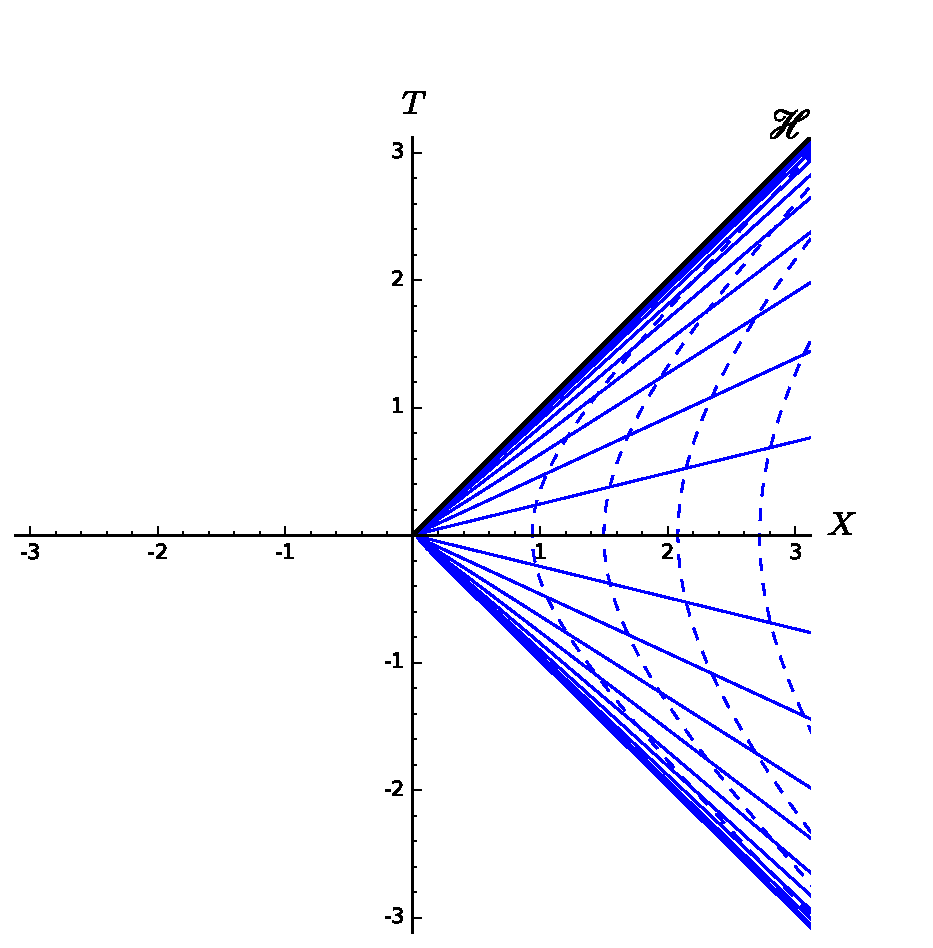
\includegraphics[width=0.6\textwidth]{sch_SD_I_KS.pdf}}
\caption[]{\label{f:sch:SD_I_KS} \footnotesize
Submanifold $\M_{\rm I}$ in the Kruskal-Szekeres coordinates $(T,X)$:
$\M_{\rm I}$ is covered by the Schwarzschild-Droste grid (in blue): the solid
lines have $t=\mathrm{const}$ (spaced apart by $\delta t = m$), while the
dashed curves have $r=\mathrm{const}$ (spaced apart by $\delta r = m/2$).}
\end{figure}


\begin{figure}
\centerline{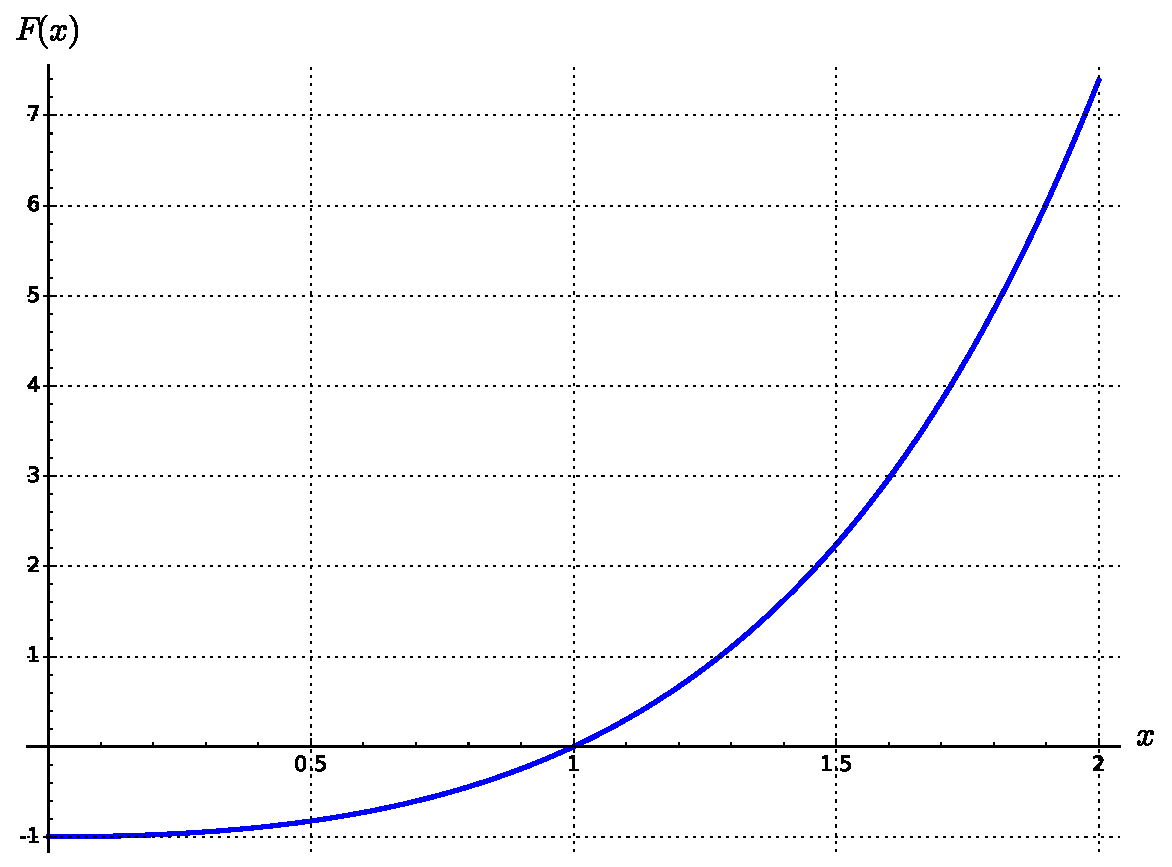
\includegraphics[height=0.37\textheight]{max_X2mT2.pdf}}
\caption[]{\label{f:max:X2mT2} \footnotesize
Function $F:\; x\mapsto \mathrm{e}^{x}(x-1)$, yielding
$X^2-T^2 = F(r/2m)$, cf. Eq.~(\ref{e:sch:X2mT2}).}
\end{figure}

We have $\D U \, \D V = (\D T - \D X) (\D T + \D X)  = \D T^2 - \D X^2$,
so that the metric components with respect to the Kruskal-Szekeres coordinates
are easily deduced from the line element (\ref{e:sch:metric_UV}):
\be \label{e:sch:metric_KS}
    \encadre{
    g_{\mu\nu} \, \D X^\mu \, \D X^\nu =
    \frac{32 m^3}{r} \, \mathrm{e}^{-r/2m}
    \left( - \D T^2 + \D X^2 \right)
     +  r^2 \left( \D\th^2 + \sin^2\th\, \D\ph^2 \right) }.
\ee
Here $r$ is to be considered as a function of $(T,X)$, which is implicitely defined
by
\be \label{e:sch:X2mT2}
   \encadre{ \mathrm{e}^{r/2m} \left( \frac{r}{2m} - 1 \right) = X^2 - T^2 } .
\ee
This relation is a direct consequence of (\ref{e:max:r_UV_M_I}) and (\ref{e:sch:def_T_X}).
We may rewrite it as
\be
    F\left( \frac{r}{2m} \right) = X^2 - T^2,
\ee
where $F$ is the function defined by
\be \label{e:sch:def_F}
    \begin{array}{cccc}
    F: & (0,+\infty) & \longrightarrow & (-1,+\infty) \\
        & x & \longmapsto & \mathrm{e}^{x}(x-1) .
    \end{array}
\ee
The graph of $F$  is shown in Fig.~\ref{f:max:X2mT2}. We see clearly that $F$ is a bijective map.
In particular, $F$ induces a bijection between $(1,+\infty)$ (the range of $r/2m$ on $\M_{\rm I}$)
and $(0,+\infty)$ (the range of $X^2-T^2$ on $\M_{\rm I}$, according to (\ref{e:sch:X_T_range_I})). The inverse of $F$ can be expressed in terms of
the \defin{Lambert function}\index{Lambert function} $W_0$, which is defined as
the inverse of $x\mapsto x \mathrm{e}^x$:
\be \label{e:sch:def_W0}
    \begin{array}{cccl}
    W_0: & (-1/\mathrm{e},+\infty) & \longrightarrow & (-1,+\infty) \\
        & x & \longmapsto & y \mbox{\ such that\ } y \mathrm{e}^{y} = x .
    \end{array}
\ee
Noticing that
\[
    F(x) = \mathrm{e}^x(x-1) = \mathrm{e}\times (x-1) \mathrm{e}^{x-1}
\]
we may write
\be
    F^{-1} = \tilde{W}_0 ,
\ee
where $\tilde{W}_0$ is the rescaled Lambert function defined by
\be \label{e:max:def_tilde_W0}
    \encadre{ \tilde{W}_0(x) := W_0\left(\frac{x}{\mathrm{e}}\right) + 1 }.
\ee
Note that $\tilde{W}_0$ is a bijection $(-1,+\infty) \to (0, +\infty)$, which
obeys
\be \label{e:max:exp_tW0}
    \mathrm{e}^{\tilde{W}_0(x)} \left( \tilde{W}_0(x) - 1 \right) = x .
\ee
Its graph is shown in Fig.~\ref{f:max:lambert_rescaled}.

\begin{figure}
\centerline{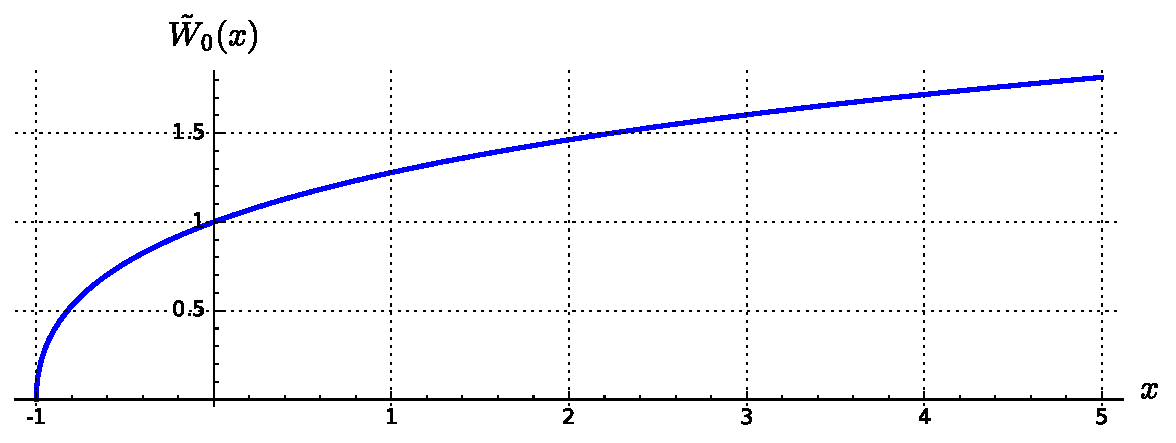
\includegraphics[width=0.8\textwidth]{max_lambert_rescaled.pdf}}
\caption[]{\label{f:max:lambert_rescaled} \footnotesize
Rescaled lambert function $\tilde{W}_0$, defined by (\ref{e:max:def_tilde_W0})
and obeying
$\mathrm{e}^{\tilde{W}_0(x)}(\tilde{W}_0(x)-1) = x$.}
\end{figure}

Using $F^{-1} = \tilde{W}_0$, we may invert the relation (\ref{e:sch:X2mT2})
to $r = 2m \tilde{W}_0(X^2-T^2)$. Noticing that
$2m/r \, \mathrm{e}^{-r/2m} = (X^2-T^2 + \mathrm{e}^{r/2m})^{-1}$
[cf. Eq.~(\ref{e:sch:X2mT2})], we may eliminate $r$ from the expression
(\ref{e:sch:metric_KS})
of the metric components in Kruskal-Szekeres coordinates:
\be \label{e:sch:metric_KS_TX_partial}
   \encadre{
    \begin{array}{lcll}
    g_{\mu\nu} \, \D X^\mu \, \D X^\nu & = & 4m^2 \bigg\{ & \displaystyle
    \frac{4}{X^2-T^2 + \mathrm{e}^{\tilde{W}_0(X^2-T^2)} }
    \left( - \D T^2 + \D X^2 \right) \\[2ex]
    & & & \displaystyle + \,   \tilde{W}_0(X^2-T^2)^2 \left( \D\th^2 + \sin^2\th\, \D\ph^2 \right)
    \bigg\}.
    \end{array} }
\ee


The relation between the Kruskal-Szekeres coordinates and the
Schwarzschild-Droste ones is obtained by combining (\ref{e:sch:def_T_X}),
(\ref{e:sch:def_U_V}) and (\ref{e:sch:u_v_r_t}):
\bea
    T &=& \frac{1}{2}(U+V) = \frac{1}{2} \left( \mathrm{e}^{v/4m}
        - \mathrm{e}^{-u/4m)} \right) =
        \frac{1}{2} \left( \mathrm{e}^{(t+r_*)/4m}
        - \mathrm{e}^{(r_*-t)/4m} \right) \nonumber \\
     & = & \mathrm{e}^{r_*/4m} \sinh\left( \frac{t}{4m} \right) ,\nonumber
\eea
where $r_*$ is related to $r$ by (\ref{e:sch:def_tortoise}).
Similarly
\[
     X = \mathrm{e}^{r_*/4m} \cosh\left( \frac{t}{4m} \right) .
\]
In particular, we have
\be \label{e:max:TsX_tanh_t}
    \frac{T}{X} = \tanh\left( \frac{t}{4m} \right) .
\ee
From Eq.~(\ref{e:sch:def_tortoise}), we have
\[
    \mathrm{e}^{r_*/4m} = \mathrm{e}^{r/4m} \sqrt{ \frac{r}{2m} - 1 } .
\]
We may summarize the above relations as follows:
\be \label{e:sch:KS_SD_I}
    \M_{\rm I}: \quad \encadre{ \left\{\begin{array}{l}
    T = \mathrm{e}^{r/4m} \sqrt{ \frac{r}{2m} - 1 } \sinh\left( \frac{t}{4m} \right)
\\[2ex]
    X = \mathrm{e}^{r/4m} \sqrt{ \frac{r}{2m} - 1 } \cosh\left( \frac{t}{4m} \right)
        \end{array}\right. }
    \iff
    \encadre{ \left\{\begin{array}{l}
    t = 2 m \,  \ln \left( \frac{X+T}{X-T} \right) \\[2ex]
    r = 2 m \tilde{W}_0(X^2 - T^2) .
        \end{array}\right. }
\ee
Note that we have used the identity $\mathrm{artanh}\, x = 1/2 \ln\left[(1+x)/(1-x)\right]$.
The curves of constant $t$ and constant $r$ in the $(T,X)$ plane
are drawn in Fig.~\ref{f:sch:SD_I_KS}.
The fact that the curves of constant $t$ are straight lines from the
origin follow immediately
from Eq.~(\ref{e:max:TsX_tanh_t}).

\begin{remark}
Given the properties of the $\cosh$ and $\sinh$ functions, it is clear on these
expressions that the constraints (\ref{e:sch:X_T_range_I}) are satisfied.
\end{remark}
\begin{remark}
In line element (\ref{e:sch:metric_KS_TX_partial})
the metric components $g_{TT}$ and $g_{XX}$ depend on both $X$ and $T$; this
shows that neither $\wpar_T$ nor $\wpar_X$ coincide with a Killing vector.
In other words, the coordinates $(T,X)$ are not adapted to the spacetime
symmetries, contrary to the Schwarzschild-Droste coordinates or to the
Eddington-Finkelstein ones.
\end{remark}

\subsection{Extension to the IEF domain}

We notice that the metric components (\ref{e:sch:metric_KS}) are perfectly
regular at $r=2m$. Therefore the Kruskal-Szekeres coordinates can be extended
to cover the Schwarzschild horizon $\Hor$. Actually they can be extended to
all values of $r\in (0,2m]$, i.e. to the whole domain of the ingoing
Eddington-Finkelstein coordinates: the manifold $\M_{\rm IEF}$ introduced
in Sec.~\ref{s:sch:Schwarz_hor}:
$\M_{\rm IEF} = \M_{\rm I} \cup \Hor \cup \M_{\rm II}$. Let us show
this in detail. Back on $\M_{\rm I}$, we can express the IEF coordinate
$\ti$ in terms of $(T,X)$ by combining $\ti = v - r$ [Eq.~(\ref{e:sch:ti_v_r})],
$v = 4m\ln V$ [Eq.~(\ref{e:sch:def_U_V})] and $V = T+X$ [Eq.~(\ref{e:sch:def_T_X})]:
\be
    \ti = 4 m \ln (T+X) - r.
\ee
The above relation is a valid expression as long as $T+X>0$.
Besides, we already noticed
that the function $F$ defined by (\ref{e:sch:def_F}) is a bijection from the range of $r/2m$
on $\M_{\rm IEF}$, i.e. $(0,+\infty)$, to $(-1,+\infty)$, with the
$(0,+\infty)$ part of the latter interval representing the range of $X^2-T^2$
on $\M_{\rm I}$. We may use these properties to extend the Kruskal-Szekeres coordinates to all $\M_{\rm IEF}$ by requiring
\begin{subequations}\label{e:sch:ti_r_X_T}
\begin{align}
 & \ti = 4 m \ln (T+X) - r\\
 & \underbrace{\mathrm{e}^{r/2m} \left( \frac{r}{2m} - 1 \right)}_{F(r/2m)} = X^2-T^2 .
 \end{align}
\end{subequations}
The range of the coordinates $(T,X)$ on $\M_{\rm IEF}$ is then ruled by
\[
    \M_{\rm IEF}:\quad T+X > 0 \quad\mbox{and}\quad X^2 - T^2 > -1 ,
\]
which can be rewritten as
\be \label{e:sch:range_X_T_IEF}
    \M_{\rm IEF}: \quad -X < T < \sqrt{X^2+1}.
\ee
We deduce from (\ref{e:sch:ti_r_X_T}) that
\be \label{e:sch:KS_IEF_prov}
    \left\{\begin{array}{lcl}
    X+T & = & \mathrm{e}^{(\ti+r)/4m} \\
    X-T & = & \mathrm{e}^{(r -\ti)/4m} \left( \frac{r}{2m} - 1 \right) .
    \end{array}\right.
\ee
Hence the relation between the ingoing Eddington-Finkelstein coordinates and
the Kruskal-Szekeres ones on $\M_{\rm IEF}$:
\be \label{e:sch:KS_IEF}
    \encadre{ \left\{\begin{array}{l}
    T = \mathrm{e}^{r/4m} \left[ \cosh\left(\frac{\ti}{4m}\right)
        - \frac{r}{4m} \mathrm{e}^{-\ti/4m} \right] \\[2ex]
    X =  \mathrm{e}^{r/4m} \left[ \sinh\left(\frac{\ti}{4m}\right)
        + \frac{r}{4m} \mathrm{e}^{-\ti/4m}  \right]
    \end{array}\right. }
    \iff
    \encadre{\left\{\begin{array}{l}
     \ti =  2 m \left[ 2 \ln (T+X) - \tilde{W}_0(X^2 - T^2) \right] \\[1ex]
    r = 2 m \tilde{W}_0(X^2 - T^2)
    \end{array}\right. }
\ee
The various subsets of $\M_{\rm IEF}$ correspond then to the following
coordinate ranges (cf. Fig.~\ref{f:sch:IEF_KS}):
\begin{subequations}
\label{e:max:range_TX_M_I_II}
\begin{align}
 & \M_{\rm I}: \quad X > 0 \quad\mbox{and}\quad -X < T < X \\
 & \Hor: \quad X > 0 \quad\mbox{and}\quad  T = X \\
 & \M_{\rm II}: \quad |X| < T < \sqrt{X^2+1} .
\end{align}
\end{subequations}

\begin{figure}
\centerline{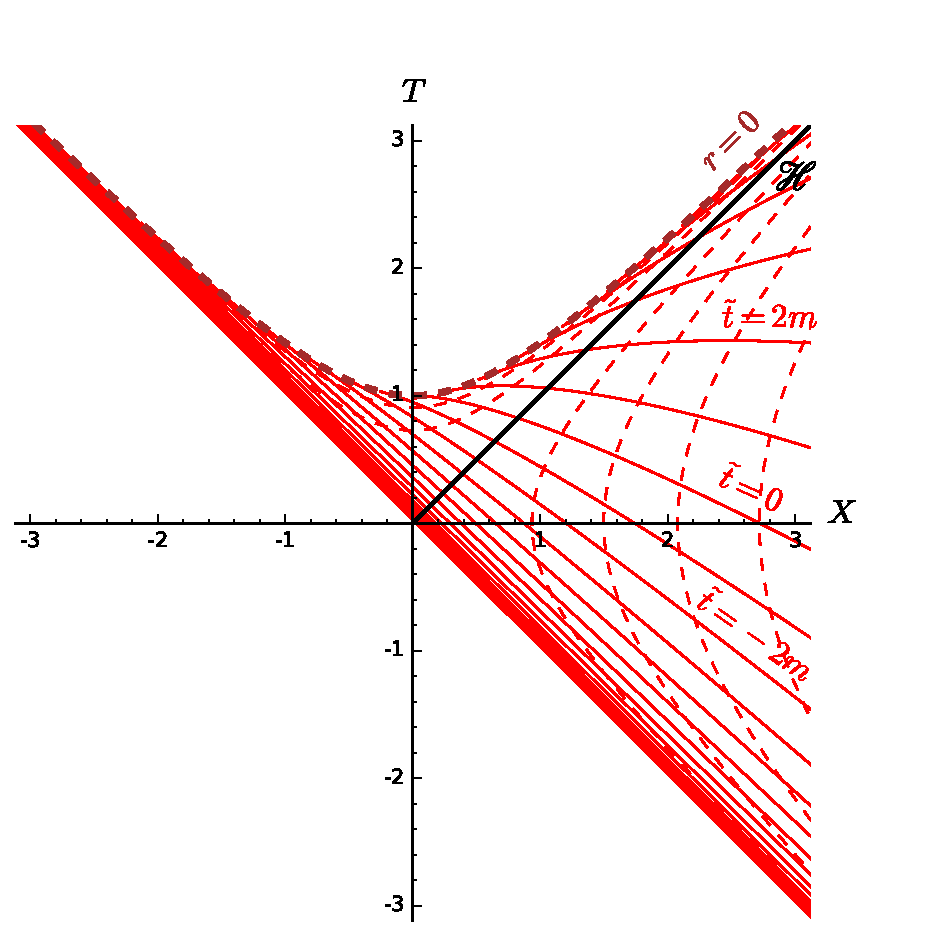
\includegraphics[width=0.6\textwidth]{sch_IEF_KS.pdf}}
\caption[]{\label{f:sch:IEF_KS} \footnotesize
Domain of ingoing Eddington-Finkelstein coordinates, $\M_{\rm IEF} = \M_{\rm I}\cup \Hor\cup \M_{\rm II}$, depicted in terms of the Kruskal-Szekeres coordinates $(T,X)$: the solid red
curves have $\ti=\mathrm{const}$ (spaced apart by $\delta\ti = m$), while the
dashed red curves have $r=\mathrm{const}$ (spaced apart by $\delta r = m/2$).}
\end{figure}


Since the relation between IEF coordinates and Kruskal-Szekeres ones is the
same in $\M_{\rm II}$ as in $\M_{\rm I}$ (being given by (\ref{e:sch:KS_IEF})
in both cases), we conclude that the expression (\ref{e:sch:metric_KS})
of the metric components with respect to
Kruskal-Szekeres coordinates is valid in all $\M_{\rm IEF}$.

Let us determine the relation between the Kruskal-Szekeres coordinates and
the Schwarz\-schild-Droste ones in $\M_{\rm II}$. Since $r<2m$ in $\M_{\rm II}$,
Eq.~(\ref{e:sch:ti_t_r}) gives
\[
    \M_{\rm II}: \quad  \mathrm{e}^{\ti/4m} = \mathrm{e}^{t/4m}  \sqrt{1 -  \frac{r}{2m} } ,
\]
so that (\ref{e:sch:KS_IEF_prov}) can be rewritten as
\[
     \M_{\rm II}: \quad
\left\{\begin{array}{lcl}
    X+T & = & \displaystyle \mathrm{e}^{(t+r)/4m} \sqrt{1 -  \frac{r}{2m} }  \\[2ex]
    X-T & = & \displaystyle  - \mathrm{e}^{(r -t)/4m}  \sqrt{1 -  \frac{r}{2m} }.
    \end{array}\right.
\]
We obtain then
\be \label{e:sch:KS_SD_II}
    \M_{\rm II}: \quad \encadre{ \left\{\begin{array}{l}
    T = \mathrm{e}^{r/4m} \sqrt{ 1 - \frac{r}{2m} } \cosh\left( \frac{t}{4m} \right)
\\[2ex]
    X = \mathrm{e}^{r/4m} \sqrt{ 1 - \frac{r}{2m} } \sinh\left( \frac{t}{4m} \right)
        \end{array}\right. }
    \iff
    \encadre{ \left\{\begin{array}{l}
    t = 2 m \,  \ln \left( \frac{T+X}{T-X} \right) \\[2ex]
    r = 2 m \tilde{W}_0(X^2 - T^2) .
        \end{array}\right. }
\ee
This is to be compared with (\ref{e:sch:KS_SD_I}).
The curves of constant $t$ and constant $r$ in the $(T,X)$ plane
are drawn in Fig.~\ref{f:sch:SD_KS}, which extends Fig.~\ref{f:sch:SD_I_KS}
to $\M_{\rm II}$.

\begin{figure}
\centerline{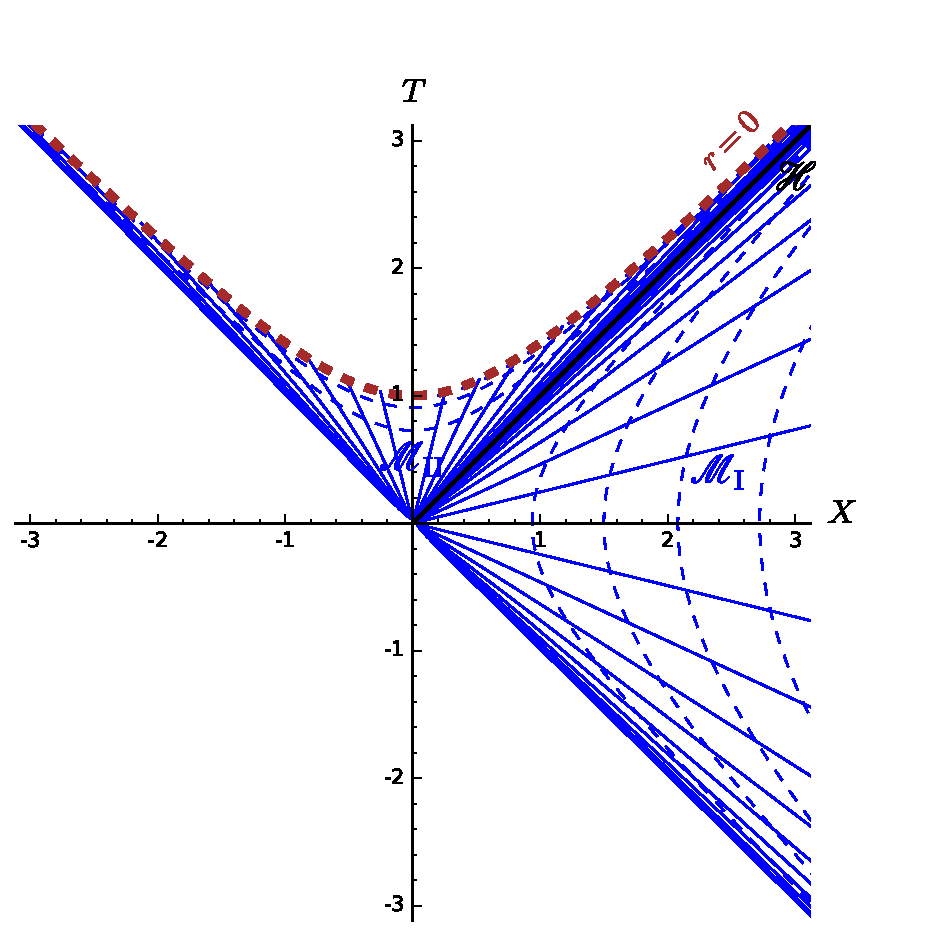
\includegraphics[width=0.6\textwidth]{sch_SD_KS.pdf}}
\caption[]{\label{f:sch:SD_KS} \footnotesize
Schwarzschild-Droste coordinates in $\M_{\rm SD} = \M_{\rm I}\cup \M_{\rm II}$
depicted in terms of the Kruskal-Szekeres coordinates $(T,X)$: the solid blue
curves have $t=\mathrm{const}$ (spaced apart by $\delta t = m$), while the
dashed blue curves have $r=\mathrm{const}$ (spaced apart by $\delta r = m/2$).}
\end{figure}


As discussed in Sec.~\ref{s:sch:singularities}, one approaches a
curvature singularity as $r\rightarrow 0$. According to (\ref{e:sch:KS_IEF})
or (\ref{e:sch:KS_SD_II}),
this corresponds to $X^2-T^2 \rightarrow -1$ (see also Fig.~\ref{f:max:X2mT2}), with
$T > 0$. Hence, in the $(T,X)$ plane, the curvature singularity is located
at $T = \sqrt{X^2 + 1}$, i.e. at the upper branch of the hyperbola
$T^2 - X^2 = 1$.

\subsection{Radial null geodesics in Kruskal-Szekeres coordinates}
\label{s:sch:rad_null_geod_KS}

By construction, the Kruskal-Szekeres coordinates $(T,X,\th,\ph)$ are
adapted to the radial null geodesics. This is clear on the expression
(\ref{e:sch:metric_KS}) of the metric tensor, where the $(T,X)$ part is
conformal to the flat metric $- \D T^2 + \D X^2$. Consequently the radial
null geodesics are straight lines of slope $\pm 45^\circ$ in the $(T,X)$ plane
(cf. Fig.~\ref{f:sch:rad_null_geod_KS}):
\begin{itemize}
\item the ingoing radial null geodesics obey
\be \label{e:sch:ingoing_null_geod_KS}
    T = - X + V ,
\ee
where $V$ is a positive constant (the constraint $V>0$ following from (\ref{e:sch:range_X_T_IEF})), so that each geodesic of this family can be labelled
by $(V,\th,\ph)$;
\item the outgoing radial null geodesics obey
\be \label{e:sch:outgoing_null_geod_KS}
    T = X + U ,
\ee
where $U$ is an arbitrary real constant, so that each geodesic of this family can be labelled
by $(U,\th,\ph)$.
\end{itemize}
\begin{figure}
\centerline{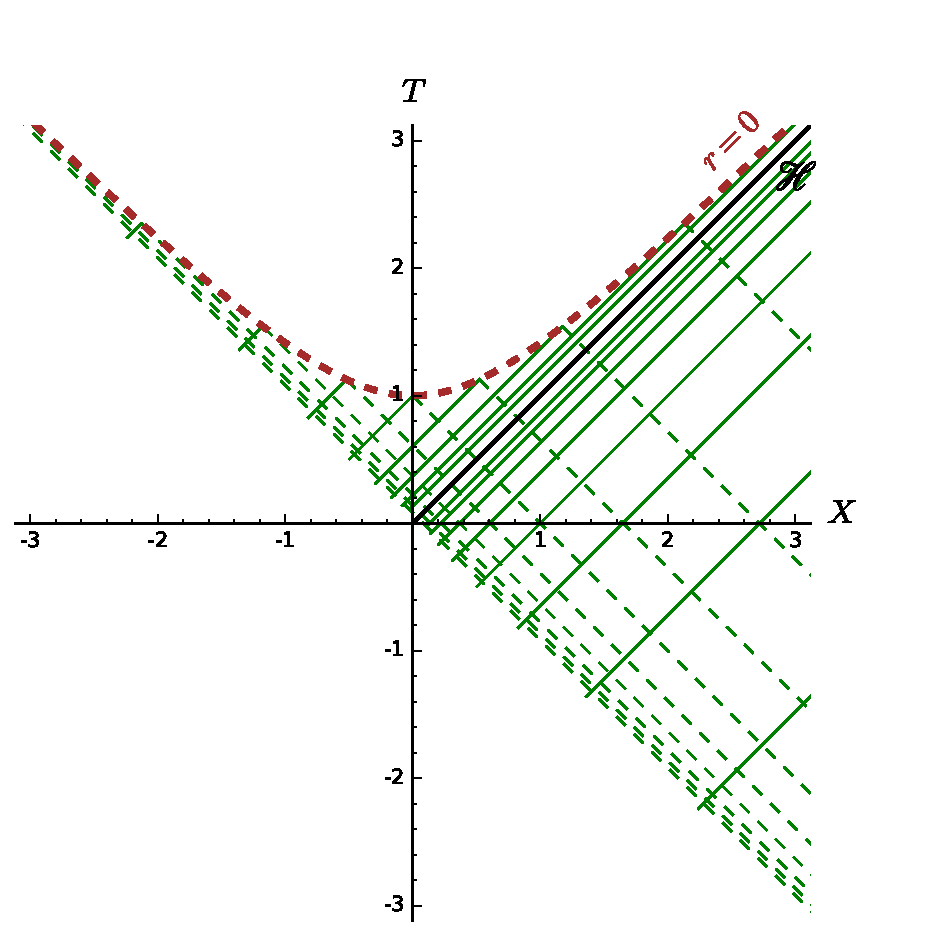
\includegraphics[width=0.6\textwidth]{sch_rad_null_geod_KS.pdf}}
\caption[]{\label{f:sch:rad_null_geod_KS} \footnotesize
Radial null geodesics in $\M_{\rm IEF} = \M_{\rm I}\cup\Hor\cup\M_{\rm II}$
depicted in terms of the Kruskal-Szekeres coordinates $(T,X)$: the solid
lines correspond to the outgoing family, with $u$ spanning $[-6m, 8m]$
(with steps $\delta u = 2m$), from the left to the right in $\M_{\rm II}$
and from the right to the left in $\M_{\rm I}$; the dashed lines
correspond to the ingoing family, with $v$ spanning $[-8m, 6m]$ (with steps $\delta v = 2m$)
from the left to the right.}
\end{figure}
In particular, the Schwarzschild horizon $\Hor$ is generated by the
outgoing radial null geodesics having $U=0$:
Eqs.~(\ref{e:sch:outgoing_null_geod_KS}) and (\ref{e:sch:X2mT2})
clearly imply $r=2m$ for $U=0$, i.e. $X=T$.
 The outgoing radial null geodesics not lying on $\Hor$ have an equation
in terms of the IEF coordinates given by
Eq.~(\ref{e:sch:outgoing_null_geod_EF}):
$\ti = r + 4 m \ln \left|r/2m- 1 \right| + u$,
where the constant $u$ is related to $U$ by
\begin{subequations}
\begin{align}
 & U = - \mathrm{e}^{-u/4m} \quad \mbox{on}\ \M_{\rm I} \\
 & U = 0 \quad \mbox{on}\ \Hor \\
 & U =  \mathrm{e}^{-u/4m} \quad \mbox{on}\ \M_{\rm II} .
\end{align}
\end{subequations}
These relations are easily established by combining
(\ref{e:sch:outgoing_null_geod_EF}) and (\ref{e:sch:KS_IEF}).


\begin{remark}
The relation $U = - \mathrm{e}^{-u/4m}$ introduced in Sec.~\ref{s:sch:KS_coord}
by Eq.~(\ref{e:sch:def_U_V}) is thus valid only in $\M_{\rm I}$. On the
contrary the relation $V = \mathrm{e}^{v/4m}$ is valid in all $\M_{\rm IEF}$.
\end{remark}

\section{Maximal extension} \label{s:sch:max_extens}

\subsection{Construction} \label{s:sch:max_extens_constr}

The spacetime $(\M_{\rm IEF}, \w{g})$ is not geodesically complete\index{geodesically complete}\index{complete!geodesically -- spacetime} (cf. Sec.~\ref{s:geo:existence_uniqueness} in Appendix~\ref{s:geo}).
Indeed, let us consider the radial null geodesics discussed above.
We have seen in Sec.~\ref{s:sch:rad_null_geod} that $r$ is an affine parameter
along them, except for those that are null generators of $\Hor$
(the outgoing ones with $U=0$).
Now, for the ingoing radial null geodesics, $r$ is decreasing towards the
future and all of them terminate at $r=0$ (the left end-point of the dashed
lines in Fig.~\ref{f:sch:rad_null_geod_KS}).
They are thus incomplete geodesics. However, they cannot be extended to
negative values of the affine parameter $r$ by extending the spacetime
since $r=0$ marks a spacetime singularity (cf. Sec.~\ref{s:sch:singularities}).

On the other hand, the outgoing radial null geodesics are limited by
the constraint $T+X > 0$, which corresponds to $r>2m$ in $\M_{\rm I}$, with $r$ increasing towards
the future, and to
$r<2m$ in $\M_{\rm II}$, with $r$ decreasing towards the future.
Thus all outgoing radial null geodesics terminate towards the past at the finite
value $2m$ of the affine parameter $r$
(the left end point of the solid lines in Fig.~\ref{f:sch:rad_null_geod_KS}) and are therefore incomplete geodesics.
However, contrary to ingoing radial null geodesics, they can be extended
since $r=2m$ does not mark any spacetime singularity.
More precisely, the limit at which outgoing radial null geodesics
terminate is $T=-X$, which by virtue of (\ref{e:sch:X2mT2}) yields $r=2m$.
This does not correspond to the Schwarzschild horizon $\Hor$, since for
the latter $T=X$, but rather to $\ti\rightarrow-\infty$,
as it is clear when comparing Fig.~\ref{f:sch:rad_null_geod_KS}
with Fig.~\ref{f:sch:IEF_KS}.

Another hint regarding the extendability of $(\M_{\rm IEF}, \w{g})$
is the fact that the Killing horizon $\Hor$ is non-degenerate, having
a non-zero surface gravity (cf. Sec.~\ref{s:neh:classif_KH}); the latter
has been computed in Example~\ref{x:def:Schw_hor3} of Chap.~\ref{s:def}:
$\kappa = 1/4m$. Now, we have seen in Sec.~\ref{s:sta:bifur_Killing_hor}
that non-degenerate Killing horizons have incomplete null generators
and, if they can be extended, they must be part of a
bifurcate Killing horizon. In the present case, the null generators of $\Hor$
are nothing but outgoing radial null geodesics. They are thus as incomplete
as those that admit $r$ as an affine parameter discussed above.

The possibility of spacetime extension beyond $\M_{\rm IEF}$ is clear
on the metric element (\ref{e:sch:metric_KS_TX_partial}): it is invariant by
the transformation
\be \label{e:sch:origin_reflection}
    \begin{array}{lccc}
    \Phi : & \R^2 & \longrightarrow & \R^2 \\
        & (T,X) & \longmapsto & (-T,-X) .
    \end{array}
\ee
Thus we may include
the part $T+X<0$ by adding a copy of $\M_{\rm IEF}$, symmetric to the
original one with respect to the ``origin'' $(T,X)=(0,0)$.
The whole spacetime manifold is then the following open subset of
$\R^2\times\mathbb{S}^2$:
\be \label{e:sch:def_M_extend}
    \encadre{ \M := \{ p \in \R^2\times\mathbb{S}^2, \quad T^2(p) - X^2(p) < 1 \} },
\ee
where $(T,X,\th,\ph)$ is the canonical coordinate system on $\R^2\times\mathbb{S}^2$,
called in this context
\defin{Kruskal-Szekeres coordinates}\index{Kruskal-Szekeres!coordinates}.
The metric $\w{g}$ on the whole $\M$ is then defined by (\ref{e:sch:metric_KS_TX_partial}):
\be \label{e:sch:metric_KS_TX}
   \encadre{
    \begin{array}{lcll}
    g_{\mu\nu} \, \D X^\mu \, \D X^\nu & = & 4m^2 \bigg\{ & \displaystyle
    \frac{4}{X^2-T^2 + \mathrm{e}^{\tilde{W}_0(X^2-T^2)} }
    \left( - \D T^2 + \D X^2 \right) \\[2ex]
    & & & \displaystyle + \,   \tilde{W}_0(X^2-T^2)^2 \left( \D\th^2 + \sin^2\th\, \D\ph^2 \right)
    \bigg\} ,
    \end{array} }
\ee
where $\tilde{W}_0$ is the rescaled Lambert function defined by
(\ref{e:max:def_tilde_W0}) (cf. Fig.~\ref{f:max:lambert_rescaled}); it is the inverse of the function
$x\mapsto \mathrm{e}^{x} (x-1)$,
which establishes a bijection from $(0,+\infty)$ to $(-1,+\infty)$.

\begin{figure}
\centerline{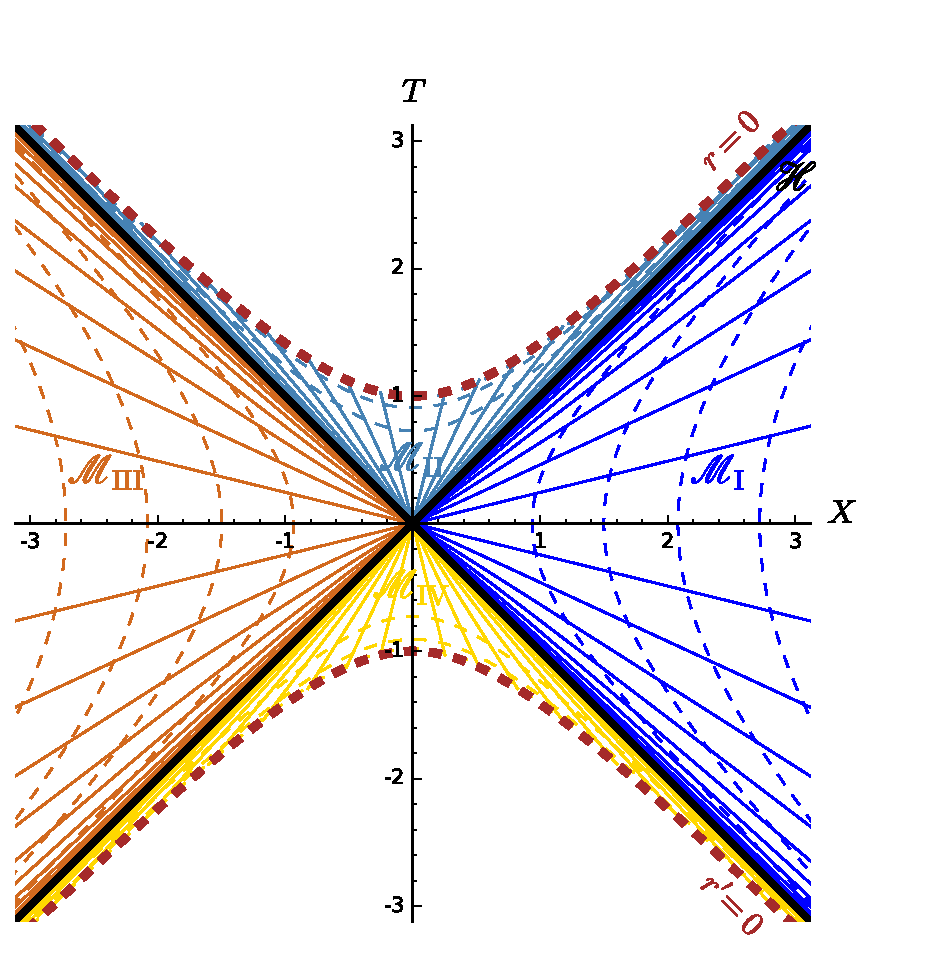
\includegraphics[width=0.6\textwidth]{sch_kruskal_diag.pdf}}
\caption[]{\label{f:sch:kruskal_diag} \footnotesize
\emph{Kruskal diagram:}
Schwarzschild spacetime $\M$ depicted in terms of Kruskal-Szekeres coordinates $(T,X)$.
Each point in this diagram, including the one at $(T,X)=(0,0)$,
is actually a sphere $\SS^2$, spanned by the
coordinates $(\th,\ph)$.
Solid lines denote the hypersurfaces $t=\mathrm{const}$ in $\M_{\rm I}$ and
$\M_{\rm II}$ and the  hypersurfaces $t'=\mathrm{const}$ in $\M_{\rm III}$ and
$\M_{\rm IV}$, whiles dashed curves
denote the hypersurfaces $r=\mathrm{const}$ in $\M_{\rm I}$ and
$\M_{\rm II}$ and the  hypersurfaces $r'=\mathrm{const}$ in $\M_{\rm III}$ and
$\M_{\rm IV}$.
The bifurcate Killing horizon is marked by thick black lines, while the
singularities at $r=0$ and $r'=0$ are depicted by the heavy dashed brown curve.}
\end{figure}

Let us define the following open subsets of $\M$, which are respectively
the images of $\M_{\rm I}$ and $\M_{\rm II}$ by the reflection through the origin
(\ref{e:sch:origin_reflection}):
\begin{subequations}
\label{e:max:range_TX_M_III_IV}
\begin{align}
 & \M_{\rm III}: \quad X < 0 \quad\mbox{and}\quad X < T < -X \\
 & \M_{\rm IV}: \quad - \sqrt{X^2+1} < T < -|X| .
\end{align}
\end{subequations}
On $\M_{\rm III}\cup \M_{\rm IV}$, one may introduce coordinates
$(t',r',\th,\ph)$ of Schwarzschild-Droste type; they are related to
the Kruskal-Szekeres coordinates by formulas analogous to
(\ref{e:sch:KS_SD_I}) and (\ref{e:sch:KS_SD_II}), simply changing $T$ to $-T$
and $X$ to $-X$:
\be \label{e:sch:KS_SD_III}
    \M_{\rm III}: \quad \encadre{ \left\{\begin{array}{l}
    T = - \mathrm{e}^{r'/4m} \sqrt{ \frac{r'}{2m} - 1 } \sinh\left( \frac{t'}{4m} \right)
\\[2ex]
    X = - \mathrm{e}^{r'/4m} \sqrt{ \frac{r'}{2m} - 1 } \cosh\left( \frac{t'}{4m} \right)
        \end{array}\right. }
    \iff
    \encadre{ \left\{\begin{array}{l}
    t' = 2 m \,  \ln \left( \frac{X+T}{X-T} \right) \\[2ex]
    r' = 2 m \tilde{W}_0(X^2 - T^2) .
        \end{array}\right. }
\ee
\be \label{e:sch:KS_SD_IV}
    \M_{\rm IV}: \quad \encadre{ \left\{\begin{array}{l}
    T = - \mathrm{e}^{r'/4m} \sqrt{ 1 - \frac{r'}{2m} } \cosh\left( \frac{t'}{4m} \right)
\\[2ex]
    X = - \mathrm{e}^{r'/4m} \sqrt{ 1 - \frac{r'}{2m} } \sinh\left( \frac{t'}{4m} \right)
        \end{array}\right. }
    \iff
    \encadre{ \left\{\begin{array}{l}
    t' = 2 m \,  \ln \left( \frac{T+X}{T-X} \right) \\[2ex]
    r' = 2 m \tilde{W}_0(X^2 - T^2) .
        \end{array}\right. }
\ee

The extended Schwarzschild spacetime $(\M,\w{g})$ is depicted in
Fig.~\ref{f:sch:kruskal_diag}, which is usually called a
\defin{Kruskal diagram}\index{Kruskal!diagram}.
There are two curvature singularities, which formally are not part of $\M$:
the hypersurfaces $r=0$ and $r'=0$.
As discussed in Sec.~\ref{s:sch:rad_null_geod_KS}, the radial null
geodesics appear as straight lines of slope $\pm 45^\circ$ ($+$ for the
outgoing family, and $-$ for the ingoing one).
As in $(\M_{\rm IEF},\w{g})$, they are still not complete but the only
locations where they terminate are the curvature singularities
at $r=0$ (future end point) and $r'=0$ (past end point). Therefore, they cannot
be extended further. For this reason, $(\M,\w{g})$ is called the
\defin{maximal extension}\index{maximal!extension}\index{extension!maximal --}
of Schwarzschild spacetime.

\begin{remark}
The extended manifold $\M$ is not just the union
$\M_{\rm I}\cup\M_{\rm II}\cup\M_{\rm III}\cup\M_{\rm IV}$, since the latter
does not cointain the hypersurfaces $T=\pm X$ (cf. the scrict inequalities
in Eqs.~(\ref{e:max:range_TX_M_I_II})
and (\ref{e:max:range_TX_M_III_IV})), which are parts of $\M$ according to
the definition (\ref{e:sch:def_M_extend}). Actually, we have
\be
    \M = \M_{\rm I}\cup\M_{\rm II}\cup\M_{\rm III}\cup\M_{\rm IV}\cup\hat{\Hor},
\ee
where $\hat{\Hor}$ is the bifurcate Killing horizon, to be discussed in
Sec.~\ref{s:max:bifur_Kill_hor}.
\end{remark}

\subsection{Global null coordinates} \label{s:max:glo_null}

In Secs.~\ref{s:sch:KS_coord} and \ref{s:sch:rad_null_geod_KS}, we have introduced
on $\M_{\rm IEF}$
the null coordinates $(U,V)$; they are related to the coordinates $(T,X)$
by Eq.~(\ref{e:sch:def_T_X}) (or equivalently
Eqs.~(\ref{e:sch:ingoing_null_geod_KS})-(\ref{e:sch:outgoing_null_geod_KS})),
which we case use define $(U,V)$ in all the maximal extension $\M$:
\be \label{e:max:U_V_T_X}
    \left\{\begin{array}{l}
    U = T - X\\
    V = T + X
    \end{array}\right.
    \qquad \iff\qquad
    \left\{\begin{array}{l}
    T = \frac{1}{2} (U+V) \\[1ex]
    X = \frac{1}{2} (V-U)
    \end{array}\right.
\ee
The range of $(U,V)$ of $\M$ is deduced from the constraint
$T^2-X^2 < 1$ [cf. Eq.~(\ref{e:sch:def_M_extend})]: since $T^2-X^2 = UV$,
we get:
\be \label{e:max:range_UV}
    \M:\quad (U,V)\in\R^2 \quad\mbox{and}\quad UV < 1.
\ee

The expression of the metric tensor
in terms of the null coordinates $x^\alpha = (U,V,\th,\ph)$
is deduced from (\ref{e:sch:metric_KS_TX}):
\be
    \encadre{
      g_{\mu\nu} \, \D x^\mu \, \D x^\nu = 4m^2 \left[
      \frac{4}{UV + \mathrm{e}^{\tilde{W}_0(-UV)} } \, \D U \, \D V
      + \tilde{W}_0(-UV)^2 \left( \D\th^2 + \sin^2\th\, \D\ph^2 \right) \right] .
    }
\ee
We can also rewrite it as (\ref{e:sch:metric_UV}):
\be \label{e:max:metric_UV_glob}
    \encadre{
    g_{\mu\nu} \, \D x^\mu \, \D x^\nu =
    - \frac{32 m^3}{r} \, \mathrm{e}^{-r/2m} \,  \D U \, \D V
     +  r^2 \left( \D\th^2 + \sin^2\th\, \D\ph^2 \right) },
\ee
where $r$ is the function of $(U,V)$ given by
\be \label{e:max:r_W0_UV}
    r = 2 m \tilde{W}_0(-UV) .
\ee
Note that the relation (\ref{e:max:r_UV_M_I}) between $r$ and $(U,V)$ holds
in all $\M$:
\be \label{e:max:r_UV}
    \encadre{ \mathrm{e}^{r/2m} \left( \frac{r}{2m} - 1 \right) = - U V } .
\ee

\begin{remark}
In Sec.~\ref{s:sch:max_extens_constr}, we have distinguished the
coordinate
$r$ in $\M_{\rm I}\cup \M_{\rm II}$ from the coordinate $r'$ in
$\M_{\rm III}\cup \M_{\rm IV}$. Here, $r$ is the function
(\ref{e:max:r_W0_UV}) of $(U,V)$, which has the same expression in
$\M_{\rm I}\cup \M_{\rm II}$ and $\M_{\rm III}\cup \M_{\rm IV}$. There is
no need to make any distinction. Hence there is no mention of $r'$
in (\ref{e:max:metric_UV_glob}).
\end{remark}


\begin{hist}
\label{n:max:KS_coord}
The Kruskal-Szekeres coordinates have been introduced in 1960 independently
by Martin D. Kruskal \cite{Krusk60} and George Szekeres \cite{Szeke60}.
Actually the coordinates
introduced by Szekeres were\footnote{They are denoted by $(v,u)$ in Szekeres' article \cite{Szeke60}.} $(2T/\sqrt{\mathrm{e}}, 2X/\sqrt{\mathrm{e}})$. Both Kruskal and Szekeres
have used these coordinates to construct the maximal  extension of Schwarzschild
spacetime. Its graphical representation in the $(X,T)$ plane (the
\emph{Kruskal diagram}\index{Kruskal!diagram}, cf. Fig.~\ref{f:sch:kruskal_diag}) has been presented by
Kruskal (Fig. 2 of Ref.~\cite{Krusk60}).
Actually, the maximal extension of Schwarzschild spacetime has been first constructed
by John L. Synge in 1950 \cite{Synge50}. He used coordinates\index{Synge!coordinates}
$(T',X')$
whose relation to
Schwarzschild-Droste coordinates is more complicated than the Kruskal-Szekeres one:
$T' = R(r) \sinh \left(\frac{t}{4m}\right)$
and $X' = R(r) \cosh \left(\frac{t}{4m}\right)$, with
$R(r) := 2m \left[ \mathrm{acosh}\sqrt{\frac{r}{2m}} + \sqrt{ \frac{r}{2m}\left(\frac{r}{2m} - 1 \right) }\right]$; compare with (\ref{e:sch:KS_SD_I}).
Albeit looking complicated, $R(r)$ is nothing but the primitive vanishing at
$r=2m$ of $r\mapsto \left(\frac{r}{2m} - 1 \right) ^{-1/2}$.
Interestingly, in his
article \cite{Szeke60}, Szekeres says that the transformations (\ref{e:sch:KS_SD_I})
``are essentially due to Synge'', probably because they differ only in the choice
of the function $R(r)$, the latter being
$R_{\rm KS}(r) = \mathrm{e}^{r/4m} \sqrt{r/2m-1}$ for Kruskal-Szekeres coordinates.
For this reason, both coordinate systems share some similarities: in Synge diagram\index{Synge!diagram} (Figs.~8 and 9 in Ref.~\cite{Synge50}),
the bifurcate horizon appears as the two bisector lines $T' = \pm X'$ and
the singularity $r=0$ as the hyperbola $T'^2 - X'^2 = \pi^2 m^2$ (compare with
$T^2-X^2 = 1$ for Kruskal-Szekeres coordinates). A major difference is that
Synge diagram is not ``conformal'': the radial null geodesics are generally not
lines with $\pm 45^\circ$ slope. Even, in some regions, the coordinate $T'$
ceases to be timelike\footnote{We refer the reader to Fig.~2 of Ref.~\cite{Unruh14}
for a plot of Synge coordinates in terms of Kruskal-Szekeres ones}.
The maximal extension of Schwarzschild spacetime
has also been found by Christian Fronsdal \cite{Frons59} in 1959, not via any explicit change of coordinates but rather via
an isometric embedding of the spacetime in the 6-dimensional Minkowski spacetime.
\end{hist}

%%%%%%%%%%%%%%%%%%%%%%%%%%%%%%%%%%%%%%%%%%%%%%%%%%%%%%%%%%%%%%%%%%%%%%%%%%%%%%%

\section{Bifurcate Killing horizon} \label{s:max:bifur_Kill_hor}

As discussed in Sec.~\ref{s:sch:max_extens}, the Schwarzschild horizon
$\Hor$ is
a non-degenerate Killing horizon and therefore shall be part of
a bifurcate Killing horizon (cf. Sec.~\ref{s:sta:bifur_Killing_hor})
in the extended spacetime.
The bifurcate Killing horizon, $\hat{\Hor}$ say, is easily found by
considering the Killing vector field $\w{\xi}$ in the maximal extension
of Schwarzschild spacetime. The components of $\w{\xi}$ w.r.t. to the
Kruskal-Szekeres coordinates are obtained from the
property $\w{\xi} = \wpar_t$:
\[
    \xi^T = \der{T}{t}, \quad
    \xi^X = \der{X}{t}, \quad
    \xi^\th = \der{\th}{t} = 0, \quad
    \xi^\ph = \der{\ph}{t} = 0 .
\]
Given the coordinate transformation laws (\ref{e:sch:KS_SD_I})
and (\ref{e:sch:KS_SD_II}), we get in
$\M_{\rm I}$ and $\M_{\rm II}$:
\[
    \xi^T = \frac{1}{4m} \, X, \quad
    \xi^X = \frac{1}{4m} \, T , \quad
    \xi^\th = \xi^\ph = 0 .
\]
Hence in $\M_{\rm I}\cup\M_{\rm II}$,
\be \label{e:sch:xi_X_T}
    \encadre{ \w{\xi} = \frac{1}{4m} \left( X \, \wpar_T + T \, \wpar_X \right) }.
\ee
Now, this formula defines a smooth vector field in all $\M$.
Moreover, in $\M_{\rm III}\cup\M_{\rm IV}$, this vector coincides with
$\wpar_{t'}$ since $\xi^T = \dert{T}{t'}$ and $\xi^X = \dert{X}{t'}$,
with the partial derivatives with respect to $t'$ evaluated from
(\ref{e:sch:KS_SD_III})-(\ref{e:sch:KS_SD_IV}). Hence the vector field
$\w{\xi}$ defined by (\ref{e:sch:xi_X_T}) is a Killing vector field
of maximal extension $(\M,\w{g})$. This vector field is depicted in
Fig.~\ref{f:sch:xi_extend}.

\begin{figure}
\centerline{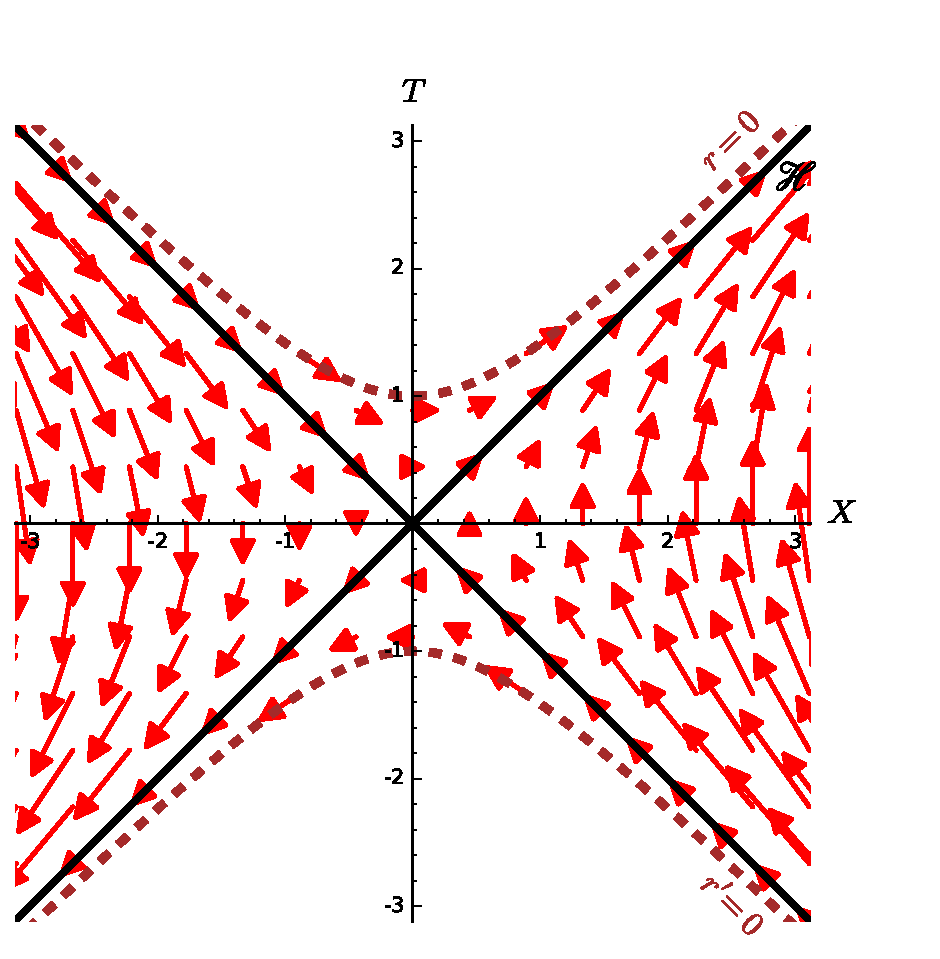
\includegraphics[width=0.6\textwidth]{sch_xi_extend.pdf}}
\caption[]{\label{f:sch:xi_extend} \footnotesize
Killing vector field $\w{\xi}$ on the extended Schwarzschild manifold.}
\end{figure}

The bifurcate Killing horizon with respect to $\w{\xi}$
that extends $\Hor$
is $\hat{\Hor} = \Hor_1 \cup \Hor_2 $, where
\begin{itemize}
\item $\Hor_1$ is the null hypersurface $T=X$ (or equivalently $U=0$);
\item $\Hor_2$ is the null hypersurface $T=-X$ (or equivalently $V=0$).
\end{itemize}
The bifurcate Killing horizon $\hat{\Hor}$ is depicted in black in
Fig.~\ref{f:sch:xi_extend}.
The Schwarzschild horizon $\Hor$ is the part of $\Hor_1$ defined by $X>0$.
In terms of the null coordinates $(U,V)$ introduced in Sec.~\ref{s:max:glo_null},
we have, given (\ref{e:max:U_V_T_X}),
\begin{subequations}
\label{e:max:Hor_U_V}
\begin{align}
    \hat{\Hor}:\quad&  U = 0 \quad\mbox{or}\quad V = 0 \\
    \Hor:\quad &   U = 0 \quad\mbox{and}\quad V > 0 .
\end{align}
\end{subequations}
The bifurcation surface is $\Sp = \Hor_1 \cap \Hor_2$, which
is the 2-surface defined by $T=0$ and $X=0$, or equivalently by
$U=0$ and $V=0$. It is a 2-sphere, since
any fixed value of the pair $(T,X)$ defines a 2-sphere, according to the
definition of $\M$ as a part of $\R^2\times\mathbb{S}^2$
[cf. Eq.~(\ref{e:sch:def_M_extend})]. Accordingly, $\Sp$ is called the
\defin{bifurcation sphere}\index{bifurcation!sphere}. It is located at the
center of Fig.~\ref{f:sch:xi_extend}.
The areal radius of $\Sp$ is found by setting
$\D T = 0$, $\D X = 0$ and $(T,X)=(0,0)$ in the line element
(\ref{e:sch:metric_KS_TX}):
\[
    r_{\Sp}^2 = 4m^2 \tilde{W}_0(0)^2.
\]
Since $\tilde{W}_0(0)=1$ (cf. Fig.~\ref{f:max:lambert_rescaled}), we get
\be
    \encadre{r_{\Sp} = 2 m } .
\ee
Moreover, setting $(T,X)=(0,0)$ in Eq.~(\ref{e:sch:xi_X_T}),
we recover the general property (\ref{e:sta:xi_S_zero}): the Killing
vector field vanishes at the bifurcation sphere:
\be
\left. \w{\xi} \right| _{\Sp} = 0 .
\ee

%%%%%%%%%%%%%%%%%%%%%%%%%%%%%%%%%%%%%%%%%%%%%%%%%%%%%%%%%%%%%%%%%%%%%%%

\section{Carter-Penrose diagram} \label{s:max:Carter-Penrose}

\subsection{First construction}

To have a compact representation of the maximal extension of Schwarzschild spacetime,
one can use the same trick as for Minkowski spacetime (cf. Sec.~\ref{s:glo:finite_range_Mink}), namely employ the arctangent function to map the
range $(-\infty, +\infty)$ of the null coordinates $U$ and $V$ to the
interval $(-\pi/2,\pi/2)$, thereby defining the finite-range coordinates
$(\hat{U},\hat{V})$:
\be \label{e:max:def_hUhV}
    \left\{ \begin{array}{l}
    \hat{U} = \arctan U \\
    \hat{V} = \arctan V
    \end{array} \right.
    \iff
   \left\{ \begin{array}{l}
    U = \tan \hat{U} \\
    V = \tan \hat{V} .
    \end{array} \right.
\ee
The range of $(\hat{U},\hat{V})$ is deduced from (\ref{e:max:range_UV}):
\[
    UV < 1 \iff \tan \hat{U} \,  \tan \hat{V} < 1 .
\]
Since for $\hat{U}, \hat{V}\in (-\pi/2,\pi/2)$, we have $\cos\hat{U} > 0$ and
$\cos\hat{V} > 0$, we may write
\[
    UV < 1 \iff  \sin\hat{U} \, \sin\hat{V} < \cos\hat{U} \, \cos\hat{V}
     \iff  \cos(\hat{U}+\hat{V}) > 0
     \iff  -\frac{\pi}{2} < \hat{U}+\hat{V} <\frac{\pi}{2} .
\]
Hence the range of $(\hat{U},\hat{V})$ on the maximal extension
of Schwarzschild spacetime:
\be \label{e:max:range_hUhV}
    \M:\quad -\frac{\pi}{2} < \hat{U} <\frac{\pi}{2},\quad
    -\frac{\pi}{2} < \hat{V} <\frac{\pi}{2}
    \quad\mbox{and}\quad -\frac{\pi}{2} < \hat{U}+\hat{V} <\frac{\pi}{2} .
\ee

Since (\ref{e:max:def_hUhV}) yields
$\D U = \D \hat{U} / \cos^2\hat{U}$ and $\D V = \D \hat{V} / \cos^2\hat{V}$,
we deduce immediately from (\ref{e:max:metric_UV_glob})
the expression of the metric tensor in terms of the coordinates
$x^\alpha = (\hat{U}, \hat{V}, \th,\ph)$:
\be \label{e:max:metric_hUhV}
    \encadre{
    g_{\mu\nu} \, \D x^\mu \, \D x^\nu =
    - \frac{32 m^3}{r} \, \mathrm{e}^{-r/2m} \,
        \frac{\D \hat{U}}{\cos^2\hat{U}} \, \frac{\D \hat{V}}{\cos^2\hat{V}}
     +  r^2 \left( \D\th^2 + \sin^2\th\, \D\ph^2 \right) },
\ee
where [cf. Eq.~(\ref{e:max:r_W0_UV})]
\be \label{e:max:r_hUhV}
    r = 2 m \tilde{W}_0(-\tan \hat{U} \tan \hat{V}) .
\ee

To depict $\M$, let us introduce  ``time+space'' coordinates $(\hat{T},\hat{X})$,
which are related to $(\hat{U},\hat{V})$ in exactly the same way
as the coordinates $(\tau,\chi)$ were related
to the finite-range null coordinates $(U,V)$ for Minkowski spacetime
[cf. Eq.~(\ref{e:glo:tau_chi_U_V})]:
\be \label{e:max:hThX_hUhV}
    \left\{ \begin{array}{l}
    \hat{T} = \hat{U} + \hat{V} \\
    \hat{X} = \hat{V} - \hat{U}
    \end{array} \right.
    \iff
    \left\{ \begin{array}{l}
    \hat{U} = \frac{1}{2} (\hat{T} - \hat{X}) \\[1ex]
    \hat{V} = \frac{1}{2} (\hat{T} + \hat{X}) .
    \end{array} \right.
\ee
The range of $(\hat{T},\hat{X})$ is deduced from (\ref{e:max:range_hUhV}):
\be \label{e:max:range_hThX}
    \M:\quad -\frac{\pi}{2} < \hat{T} <\frac{\pi}{2},\quad
        \hat{T}-\pi < \hat{X} < \hat{T}+\pi
    \quad\mbox{and}\quad -\hat{T}-\pi < \hat{X} < -\hat{T}+\pi.
\ee


Via (\ref{e:max:def_hUhV}) and (\ref{e:max:U_V_T_X}), the relation
between $(\hat{T},\hat{X})$ and the Kruskal-Szekeres coordinates $(T,X)$
is then the same as that between $(\tau,\chi)$ and $(t,r)$ for Minkowksi
spacetime [Eq.~(\ref{e:glo:tau_chi_t_r})]:
\be \label{e:max:tTtX}
    \left\{ \begin{array}{l}
    \hat{T} = \arctan(T+X) + \arctan(T-X) \\
    \hat{X} = \arctan(T+X) - \arctan(T-X)
    \end{array} \right.
    \iff
    \left\{ \begin{array}{l}
    \displaystyle T = \frac{\sin\hat{T}}{\cos\hat{T} + \cos\hat{X}}\\[2ex]
    \displaystyle X = \frac{\sin\hat{X}}{\cos\hat{T} + \cos\hat{X}} .
    \end{array} \right.
\ee

The maximal extension of Schwarzschild spacetime is depicted with respect
to the coordinates $(\hat{T},\hat{X})$ in Fig.~\ref{f:max:carter-penrose-std}.
Such a plot is called a \defin{Carter-Penrose diagram}\index{Carter-Penrose diagram}
(see the historical note p.~\pageref{h:max:CP-diag}).
As the Kruskal diagram (Fig.~\ref{f:sch:kruskal_diag}), it has the property
to display the radial null geodesics as straight lines with slope $\pm 45^\circ$.
This holds
since $\hat{U}$ (resp. $\hat{V}$) is a function of $U$ only
(resp. $V$ only), cf. Eq.~(\ref{e:max:def_hUhV}), so that $\hat{U}$
(resp. $\hat{V}$) is constant on outgoing (resp. ingoing) radial null geodesics.
In particular, the bifurcate Killing horizon and the Schwarzschild horizon
are obtained for specific values of $\hat{U}$ and $\hat{V}$:
\begin{subequations}
\begin{align}
    \hat{\Hor}:\quad&  \hat{U} = 0 \quad\mbox{or}\quad \hat{V} = 0 \\
    \Hor:\quad &  \hat{U} = 0 \quad\mbox{and}\quad \hat{V} > 0 .
\end{align}
\end{subequations}
These relations follow immediately from (\ref{e:max:Hor_U_V}) and
(\ref{e:max:def_hUhV}).


\begin{figure}
\centerline{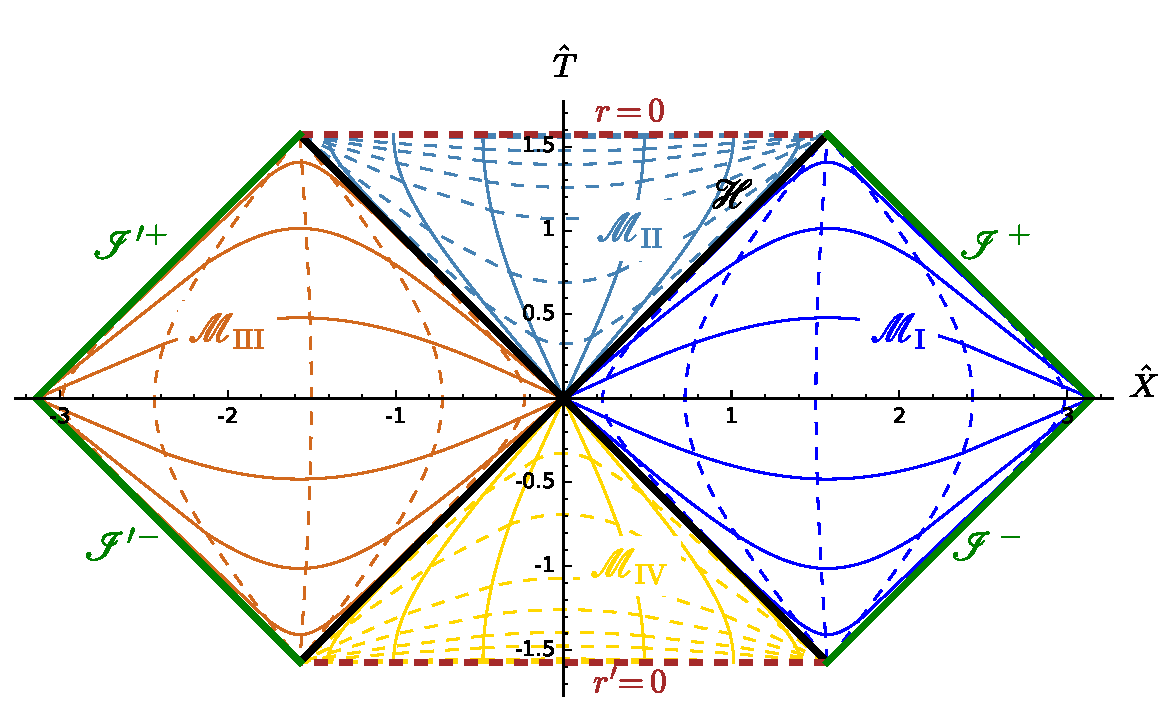
\includegraphics[width=0.9\textwidth]{max_carter-penrose-std.pdf}}
\caption[]{\label{f:max:carter-penrose-std} \footnotesize
Carter-Penrose diagram of the Schwarzschild spacetime
constructed with the compactified coordinates $(\hat{T},\hat{X})$.
Solid curves denote hypersurfaces of constant Schwarzschild-Droste coordinate
$t$: in region $\M_{\rm I}$, from the $\hat{X}$-axis to the top: $t=0$, $2m$,
$5m$, $10m$, $20m$ and $50m$, the last two being barely visible;
in region $\M_{\rm II}$, from the $\hat{T}$-axis
to the right: $t=0$, $2m$, $5m$, $10m$, $20m$ and $50m$,
Dashed curves denote hypersurfaces of constant Schwarzschild-Droste coordinate
$r$: in region $\M_{\rm I}$, from the left to the right: $r=2.01m$, $2.1m$, $2.5m$ (almost vertical), $4m$, $8m$, $12m$, $20m$ and $100m$, the last three being barely visible;
in region $\M_{\rm II}$, from the bottom to the top: $r=1.98m$, $1.9m$, $1.7m$,
$1.5m$, $1.25m$, $m$, $0.5m$ and $0.1m$.
The color code
is the same as in Fig.~\ref{f:sch:kruskal_diag}.
See Sec.~\ref{s:sam:std_Carter-Penrose} for the
SageManifolds worksheet generating this figure.}
\end{figure}


We have seen in Sec.~\ref{s:sch:BH} that the future null infinity $\scri^+$
corresponds to $v\rightarrow +\infty$ and that the past null infinity
$\scri^-$ to $u\rightarrow -\infty$ (cf. Fig.~\ref{f:sch:conf_compl_final}).
Since on $\M_{\rm I}$, $U = - \mathrm{e}^{-u/4m}$ and $V = \mathrm{e}^{v/4m}$
[cf. Eq.~(\ref{e:sch:def_U_V})], we
may write equivalently:
\begin{subequations}
\begin{align}
    \scri^+:&\quad V\rightarrow +\infty \quad\mbox{and}\quad U \in (-\infty, 0) \\
    \scri^-:&\quad U\rightarrow -\infty \quad\mbox{and}\quad V \in (0,+\infty) .
\end{align}
\end{subequations}
In view of (\ref{e:max:def_hUhV}), we get then:
\begin{subequations}
\label{e:max:scri_hUhV}
\begin{align}
    \scri^+:&\quad \hat{V}\rightarrow \frac{\pi}{2} \quad\mbox{and}\quad
        \hat{U} \in \left( -\frac{\pi}{2} , 0 \right) \\
    \scri^-:&\quad \hat{U}\rightarrow -\frac{\pi}{2} \quad\mbox{and}\quad
         \hat{V} \in \left( 0 ,  \frac{\pi}{2} \right).
\end{align}
\end{subequations}

By symmetry, the extension $\M_{\rm III}\cup \M_{\rm IV}$ of Schwarzschild
spacetime has the following null infinity:
\begin{subequations}
\label{e:max:scri_prime_hUhV}
\begin{align}
    {\scri'}^+:&\quad \hat{U}\rightarrow \frac{\pi}{2} \quad\mbox{and}\quad
        \hat{V} \in \left( -\frac{\pi}{2} , 0 \right) \\
    {\scri'}^-:&\quad \hat{V}\rightarrow -\frac{\pi}{2} \quad\mbox{and}\quad
        \hat{U}\in \left( 0 ,  \frac{\pi}{2} \right).
\end{align}
\end{subequations}

\subsection{Discussion: Carter-Penrose diagram and conformal completion}
\label{s:max:discus_hUhV}

The Carter-Penrose diagram in Fig.~\ref{f:max:carter-penrose-std} can be compared with the conformal diagram
of Minkowski spacetime in Fig.~\ref{f:glo:conf_diag_Mink}.
The right asymptotics of the Carter-Penrose diagram
(i.e. the part $\hat{X}>\pi/2$) looks similar to that of
Minkowski conformal diagram.
However, there is a difference: the coordinates $(\hat{T},\hat{X})$
employed in the construction of the diagram of
Fig.~\ref{f:max:carter-penrose-std} are not related to any (regular) conformal
completion --- as defined in Sec.~\ref{s:glo:conf_compl} ---
contrary to the coordinates $(\tau,\chi)$ used for Minkowski spacetime.

To see this, let us rewrite the metric components (\ref{e:max:metric_hUhV})
in a form that makes clear their behavior near null infinity. Given (\ref{e:max:r_hUhV}) and (\ref{e:max:exp_tW0}), we have
\be \label{e:max:exp_r_hUhV}
    \mathrm{e}^{r/2m} \left( \frac{r}{2m} - 1 \right) =
        -\tan \hat{U} \tan \hat{V} ,
\ee
from which we get
\[
    \frac{2m}{r} \mathrm{e}^{-r/2m} = - \frac{1-2m/r}{\tan \hat{U} \tan \hat{V}} .
\]
Hence
\[
    \frac{2m}{r} \frac{\mathrm{e}^{-r/2m}}{\cos^2\hat{U}\cos^2\hat{V}}
    =- \frac{1-2m/r}{\sin \hat{U} \cos\hat{U} \sin\hat{V}\cos\hat{V}}
   =  - \frac{4(1-2m/r)}{\sin 2\hat{U} \sin 2\hat{V}} .
\]
Therefore, we may rewrite expression~(\ref{e:max:metric_hUhV})
for the metric tensor as
\be \label{e:max:metric_hUhV_asymp}
    g_{\mu\nu} \, \D x^\mu \, \D x^\nu =
     64 m^2 \left( 1 - \frac{2m}{r} \right)\,
    \frac{\D \hat{U} \, \D \hat{V}}{\sin 2\hat{U} \sin 2\hat{V}}
     +  r^2 \left( \D\th^2 + \sin^2\th\, \D\ph^2 \right)  ,
\ee
with $r$ given by (\ref{e:max:r_hUhV}).
To get a conformal completion, we should write (cf. Sec.~\ref{s:glo:conf_compl})
\be \label{e:max:g_Omega2_tg}
    \w{g} = \Omega^{-2} \w{\tilde{g}} ,
\ee
where $\Omega = 0$ and $\dd\Omega \not=0$ on the spacetime boundary $\scri$ and
$\w{\tilde{g}}$ is a regular metric on the completion $\M\cup\scri$.
Since in Eq.~(\ref{e:max:metric_hUhV_asymp}), the term
$\sin 2\hat{U} \sin 2\hat{V}$ vanishes
at $\scri = \scri^+ \cup \scri^- \cup {\scri'}^+ \cup {\scri'}^-$
[cf. Eqs.~(\ref{e:max:scri_hUhV})-(\ref{e:max:scri_prime_hUhV})],
we would have, up to some constant factor,
\be \label{e:max:Omega_hUhV}
    \Omega = \sqrt{-\sin 2\hat{U} \sin 2\hat{V}} ,
\ee
the minus sign taking into account that
$\sin 2\hat{U} \sin 2\hat{V}$ approaches zero via negative values near
$\scri$.
A first issue is that the square root in (\ref{e:max:Omega_hUhV}) makes
$\Omega$ not differentiable on $\scri$, where either $\sin 2 \hat{U}=0$
or $\sin 2\hat{V}=0$. In other words, $\dd\Omega$ is diverging on $\scri$.
Suppose we accept this and are ready
to introduce a slight deviation (given that $\Omega^2$, which is involved in (\ref{e:max:g_Omega2_tg}), is smooth) from the definition given in
Sec.~\ref{s:glo:conf_compl}.
Then the conformal metric should be
\be \label{e:max:conf_metric_hUhV}
   {\tilde{g}}_{\mu\nu} \, \D x^\mu \, \D x^\nu =
     - 64 m^2 \left( 1 - \frac{2m}{r} \right)
    \D \hat{U} \, \D \hat{V}
     -  r^2 \sin 2\hat{U} \sin 2\hat{V}
     \left( \D\th^2 + \sin^2\th\, \D\ph^2 \right) .
\ee
Near $\scri$, $r\rightarrow +\infty$ and we have ${\tilde{g}}_{\hat{U}\hat{V}} \rightarrow -64 m^2$. On the contrary, ${\tilde{g}}_{\theta\theta}$ is
of the type ``$\infty\times 0$''; in order to determine its behaviour, let
us rewrite it as follows:
\[
    {\tilde{g}}_{\theta\theta} = -  r^2 \sin 2\hat{U} \sin 2\hat{V}
        = - 4 r^2 \sin\hat{U}\sin\hat{V} \times \cos\hat{U}\cos\hat{V},
\]
with $\cos\hat{U}\cos\hat{V}$ expressed via (\ref{e:max:exp_r_hUhV}):
\[
    \cos\hat{U}\cos\hat{V} = - \sin\hat{U} \sin\hat{V}
    \frac{\mathrm{e}^{-r/2m}}{r/2m - 1} .
\]
Hence
\[
    {\tilde{g}}_{\theta\theta} = 8 m \sin^2\hat{U} \sin^2\hat{V}
    \frac{ r \mathrm{e}^{-r/2m}}{1 - 2m/r}
\]
and (\ref{e:max:conf_metric_hUhV}) becomes
\be
   {\tilde{g}}_{\mu\nu} \, \D x^\mu \, \D x^\nu =
     - 64 m^2 \left( 1 - \frac{2m}{r} \right)
    \D \hat{U} \, \D \hat{V}
     + 8 m \sin^2\hat{U} \sin^2\hat{V}
    \frac{r \mathrm{e}^{-r/2m}}{1 - 2m/r}
     \left( \D\th^2 + \sin^2\th\, \D\ph^2 \right) .
\ee
On this expression, we can read directly the value of the conformal metric
at $\scri$,  where $r\rightarrow +\infty$, $2m/r \rightarrow 0$,
$r \mathrm{e}^{-r/2m}\rightarrow 0$ and
$\sin^2\hat{U}\rightarrow 1$ or
$\sin^2\hat{V}\rightarrow 1$:
\be \label{e:max:conf_metric_scri}
   {\tilde g}_{\mu\nu} \, \D x^\mu \, \D x^\nu
   \ \stackrel{\scri}{=}\  - 64 m^2 \D \hat{U} \, \D \hat{V} .
\ee
This bilinear form is clearly degenerate (cf. Sec.~\ref{s:bas:metric}).
Therefore $\w{\tilde{g}}$ is not a
regular metric on the whole manifold $\M\cup\scri$.
We conclude that (\ref{e:max:Omega_hUhV})-(\ref{e:max:conf_metric_hUhV}) does
not define a conformal completion of $(\M,\w{g})$.

\begin{hist} \label{h:max:CP-diag}
The first compactified conformal diagram of the (maximal extension of) Schwarzschild
spacetime has been constructed by Brandon Carter\index{Carter, B.} in 1965 \cite{Carte66}, using the same coordinates $(\hat{T},\hat{X})$ as here\footnote{
$(\hat{T},\hat{X})$ are denoted $(\psi,\xi)$ by Carter \cite{Carte66}.}: compare Fig.~\ref{f:max:carter-penrose-std} with Fig.~1c of Ref.~\cite{Carte66}.
In his article, Carter notes that ``the manner in which the distant flat-space
parts (...) are compressed into finite parts of the $(\xi,\psi)$ plane by the
coordinate transformations recalls the conformal diagrams used by R. Penrose''
in 1964 \cite{Penro64}, which regard Minkowski and de Sitter spacetimes only.
Hence it seems quite fair to call the graphical representation shown in Fig.~\ref{f:max:carter-penrose-std}
a \emph{Carter-Penrose diagram}\index{Carter-Penrose diagram}, and not merely
a \emph{Penrose diagram}\index{Penrose!diagram}, as often done in the literature.
\end{hist}

\subsection{A regular conformal completion based on Frolov-Novikov coordinates}
\label{s:max:regul_conf_compl}

In order to get a regular conformal completion of the maximally extended
Schwarzschild spacetime $(\M,\w{g})$, a finite-range coordinate system has
been proposed by Frolov \& Novikov \cite{FroloN98}: instead of (\ref{e:max:def_hUhV}),
the finite-range coordinates $(\tilde{U},\tilde{V})$ are defined in terms
of the null Kruskal-Szekeres coordinates $(U,V)$ by
\be \label{e:max:def_tUtV}
    \left\{ \begin{array}{l}
    \tilde{U} = \arctan(\mathrm{arsinh}\, U) \\
    \tilde{V} = \arctan(\mathrm{arsinh}\, V)
    \end{array} \right.
    \iff
   \left\{ \begin{array}{l}
    U = \sinh(\tan \tilde{U}) \\
    V = \sinh(\tan \tilde{V}) .
    \end{array} \right.
\ee
The range of $(\tilde{U},\tilde{V})$ is deduced from (\ref{e:max:range_UV}):
\be \label{e:max:range_tUtV}
    \M:\quad -\frac{\pi}{2} < \tilde{U} <\frac{\pi}{2},\quad
    -\frac{\pi}{2} < \tilde{V} <\frac{\pi}{2}
    \quad\mbox{and}\quad  \sinh(\tan \tilde{U}) \sinh(\tan \tilde{V}) < 1 .
\ee
Note that contrary to what happened for $(\hat{U},\hat{V})$, these conditions
do not yield to simple polygonal region in the $(\tilde{U},\tilde{V})$ plane.
The presence of the $\sinh$ function in the expression (\ref{e:max:def_tUtV}) of
$(U,V)$ in terms of $(\tilde{U},\tilde{V})$ does not alter the values
of the finite-range coordinates at null infinity, as compared to
$(\hat{U},\hat{V})$ [cf. (\ref{e:max:scri_hUhV})-(\ref{e:max:scri_prime_hUhV})]:
\begin{subequations}
\label{e:max:scri_tUtV}
\begin{align}
    \scri^+:&\quad \tilde{V}\rightarrow \frac{\pi}{2} \quad\mbox{and}\quad
        \tilde{U} \in \left( -\frac{\pi}{2} , 0 \right) \\
    \scri^-:&\quad \tilde{U}\rightarrow -\frac{\pi}{2} \quad\mbox{and}\quad
         \tilde{V} \in \left( 0 ,  \frac{\pi}{2} \right) \\
    {\scri'}^+:&\quad \tilde{U}\rightarrow \frac{\pi}{2} \quad\mbox{and}\quad
        \tilde{V} \in \left( -\frac{\pi}{2} , 0 \right) \\
    {\scri'}^-:&\quad \tilde{V}\rightarrow -\frac{\pi}{2} \quad\mbox{and}\quad
        \tilde{U}\in \left( 0 ,  \frac{\pi}{2} \right).
\end{align}
\end{subequations}
We shall call $(\tilde{U},\tilde{V},\th,\ph)$ the
\defin{Frolov-Novikov coordinates}\index{Frolov-Novikov coordinates}.

From (\ref{e:max:def_tUtV}), we get
\[
    \D U = \frac{\cosh(\tan\tilde{U})}{\cos^2\tilde{U}}\, \D\tilde{U}
    \qquad\mbox{and}\qquad
    \D V = \frac{\cosh(\tan\tilde{V})}{\cos^2\tilde{V}}\, \D\tilde{V} ,
\]
so that the metric components in terms of the coordinates
$x^\alpha=(\tilde{U},\tilde{V},\th,\ph)$ are easily deduced from
(\ref{e:max:metric_UV_glob})-(\ref{e:max:r_W0_UV}):
\be \label{e:max:metric_tUtV}
    \encadre{
    g_{\mu\nu} \, \D x^\mu \, \D x^\nu =
    - \frac{32 m^3}{r} \, \mathrm{e}^{-r/2m} \,
        \frac{\cosh(\tan\tilde{U}) \cosh(\tan\tilde{V})}{\cos^2\tilde{U}\cos^2\tilde{V}}\,
            \D\tilde{U} \, \D\tilde{V}
     +  r^2 \left( \D\th^2 + \sin^2\th\, \D\ph^2 \right) },
\ee
where $r$ is the function of $(\tilde{U},\tilde{V})$ given by
\be \label{e:max:r_tUtV}
    r = 2 m \tilde{W}_0\!\left(-\sinh(\tan \tilde{U}) \sinh(\tan \tilde{V})\right) .
\ee
As we did for $(\hat{U},\hat{V})$, let us rewrite (\ref{e:max:metric_tUtV}) in
a form that is better adapted to the null asymptotics.
Given (\ref{e:max:r_tUtV}) and (\ref{e:max:exp_tW0}), we have
\be \label{e:max:exp_r_tUtV}
    \mathrm{e}^{r/2m} \left( \frac{r}{2m} - 1 \right) =
        - \sinh(\tan \tilde{U}) \sinh(\tan \tilde{V}) ,
\ee
from which we get
\[
    \frac{2m}{r} \mathrm{e}^{-r/2m} = - \left( 1 - \frac{2m}{r} \right)
        \frac{1}{\sinh(\tan \tilde{U}) \sinh(\tan \tilde{V})} .
\]
Hence (\ref{e:max:metric_tUtV}) becomes
\bea
    g_{\mu\nu} \, \D x^\mu \, \D x^\nu & =&
    16 m^2 \left( 1 - \frac{2m}{r} \right)
    \frac{\D\tilde{U} \, \D\tilde{V}}{\tanh(\tan\tilde{U}) \tanh(\tan\tilde{V}) \cos^2\tilde{U}\cos^2\tilde{V}} \nonumber\\
    & &
     +  r^2 \left( \D\th^2 + \sin^2\th\, \D\ph^2 \right) .
\eea
Given the values (\ref{e:max:scri_tUtV}) of $\tilde{U}$ and $\tilde{V}$ near
$\scri$, $\tanh(\tan\tilde{U}) \tanh(\tan\tilde{V})$ does not vanish there.
A natural choice of conformal factor is then
\be \label{e:max:def_Omega_tUtV}
   \encadre{ \Omega := \cos\tilde{U}\cos\tilde{V} }.
\ee
The corresponding conformal metric is
\be \label{e:max:conf_metric_tUtV}
    \encadre{
    \begin{array}{lcl}
    \displaystyle {\tilde g}_{\mu\nu} \, \D x^\mu \, \D x^\nu & =&
    \displaystyle 16 m^2 \left( 1 - \frac{2m}{r} \right)
    \frac{\D\tilde{U} \, \D\tilde{V}}{\tanh(\tan\tilde{U}) \tanh(\tan\tilde{V}) } \\[2ex]
    & &
     +  r^2 \cos^2\tilde{U}\cos^2\tilde{V} \left( \D\th^2 + \sin^2\th\, \D\ph^2 \right)
    \end{array} } .
\ee
Considering $(\tilde{U},\tilde{V},\th,\ph)$ as a canonical coordinate system
on $\R^2\times\SS^2$, we define the conformal completion manifold as
\bea
    \tilde{\M} &:= &\left\{ p\in \R^2\times\SS^2,\  (\tilde{U}(p),\tilde{V}(p)) \in \left( -\frac{\pi}{2}, \frac{\pi}{2} \right) ^2 \ \mbox{and}\
       \sinh(\tan \tilde{U}(p)) \sinh(\tan \tilde{V}(p)) < 1 \right\}
        \nonumber \\
       & & \cup \scri^+ \cup \scri^- \cup {\scri'}^+ \cup {\scri'}^- ,
        \label{e:max:def_M_compl}
\eea
with
\begin{subequations}\label{e:max:def_scri_R2S2}
\begin{align}
   \scri^+ := &\ \left\{ p\in \R^2\times\SS^2,\  \tilde{V}(p) = \frac{\pi}{2}
        \ \mbox{and}\ \tilde{U}(p) \in \left( -\frac{\pi}{2}, 0 \right) \right\}
            \label{e:max:def_scrip_R2S2} \\
    \scri^- := &\ \left\{ p\in \R^2\times\SS^2,\  \tilde{U}(p) = -\frac{\pi}{2}
        \ \mbox{and}\ \tilde{V}(p) \in \left( 0, \frac{\pi}{2}\right) \right\} \\
   {\scri'}^+ := &\ \left\{ p\in \R^2\times\SS^2,\  \tilde{U}(p) = \frac{\pi}{2}
        \ \mbox{and}\ \tilde{V}(p) \in \left( -\frac{\pi}{2}, 0 \right) \right\} \\
   {\scri'}^- := &\ \left\{ p\in \R^2\times\SS^2,\  \tilde{V}(p) = -\frac{\pi}{2}
        \ \mbox{and}\ \tilde{U}(p) \in \left( 0, \frac{\pi}{2}\right) \right\} .
\end{align}
\end{subequations}
Note that the first line in (\ref{e:max:def_M_compl}) corresponds to $\M$,
identified as a subset of $\R^2\times\SS^2$ [cf. Eq.~(\ref{e:max:range_tUtV})]
and that the definitions of $\scri^+$, $\scri^-$, ${\scri'}^+$ and ${\scri'}^-$
are in agreement with (\ref{e:max:scri_tUtV}). It is clear that $\tilde{\M}$
is a manifold with boundary and that
\be
    \partial\tilde{\M} = \scri := \scri^+ \cup \scri^- \cup {\scri'}^+
            \cup {\scri'}^- .
\ee
Moreover the scalar field $\Omega$ defined by (\ref{e:max:def_Omega_tUtV})
satisfies $\Omega \geq 0$ on $\tilde{\M}$, along with
$\Omega = 0$ on $\scri$ and $\dd\Omega\not = 0$ on $\scri$. The last property
follows from
\[
    \dd\Omega = -\sin\tilde{U} \cos\tilde{V}\, \dd\tilde{U}
            -\cos\tilde{U} \sin\tilde{V}\, \dd\tilde{V} ,
\]
which implies
$\left.\dd\Omega\right|_{\scri^+} = -\cos\tilde{U}\, \dd\tilde{V}\not=0$,
$\left.\dd\Omega\right|_{\scri^-} = \cos\tilde{V}\, \dd\tilde{U}\not=0$,
$\left.\dd\Omega\right|_{{\scri'}^+} = -\cos\tilde{V}\, \dd\tilde{U}\not=0$ and
$\left.\dd\Omega\right|_{{\scri'}^-} = \cos\tilde{U}\, \dd\tilde{V}\not=0$.
Hence the conditions 1, 3 and 4 of the definition of a conformal completion
given in Sec.~\ref{s:glo:conf_compl} are fulfilled. There remains to check
condition 2, namely that the tensor $\w{\tilde{g}}$ defined
by (\ref{e:max:conf_metric_tUtV}) is a regular metric on the whole $\tilde{\M}$.
This was the main failing point in the attempt of Sec.~\ref{s:max:discus_hUhV}.
Since $\Omega^2 > 0$ on $\M$, $\w{\tilde{g}}$ is well behaved on $\M$. Let us
thus examine its behaviour on $\scri$. We shall focus
on $\scri^+$, the behaviour on the other parts of $\scri$ being obtained by
some trivial symmetry. As one approaches $\scri^+$, $r\rightarrow +\infty$,
$\tilde{V}\rightarrow \pi/2$ and $\tanh(\tan(\tilde{V})\rightarrow 1$;
accordingly
we read from (\ref{e:max:conf_metric_tUtV}) that
\[
    \tilde{g}_{\tilde{U}\tilde{V}}
    \ \stackrel{\scri^+}{=}\  \frac{8 m^2}{\tanh(\tan\tilde{U})} \,
    \D\tilde{U} \, \D\tilde{V} .
\]
Besides, we have
$\tilde{g}_{\th\th} = r^2 \cos^2\tilde{U}\cos^2\tilde{V}$, which is of the type
``$+\infty \times 0$'' near $\scri^+$. Noticing that
$\tan\tilde{V}\sim 1/\cos\tilde{V}$ when $\tilde{V}\rightarrow \pi/2$, we get
from (\ref{e:max:exp_r_tUtV})
\[
    \sinh\left(\frac{1}{\cos\tilde{V}}\right) \sim - \frac{r \mathrm{e}^{r/2m}}{2m\sinh(\tan\tilde{U})}
        \quad \mbox{when} \quad \tilde{V}\rightarrow \frac{\pi}{2} .
\]
Since $\mathrm{arsinh}(x) = \ln(x + \sqrt{x^2+1}) \sim \ln x$ when $x\rightarrow +\infty$,
we obtain
\bea
    \frac{1}{\cos\tilde{V}} & \sim & \ln\left( - \frac{r \mathrm{e}^{r/2m}}{2m\sinh(\tan\tilde{U})} \right)
        = \frac{r}{2m} + \ln \left( \frac{r}{2m} \right) - \ln\left(-\sinh(\tan\tilde{U})\right) \nonumber \\
        & \sim & \frac{r}{2m} \quad \mbox{when} \quad \tilde{V}\rightarrow \frac{\pi}{2} .
            \nonumber
\eea
Hence $\cos^2\tilde{V} \sim 4m^2 / r^2$ and $\tilde{g}_{\th\th} \sim 4 m^2 \cos^2\tilde{U}$.
Gathering the above results, we have
\be
   {\tilde g}_{\mu\nu} \, \D x^\mu \, \D x^\nu
   \ \stackrel{\scri^+}{=}\  4 m^2 \left[
    \frac{4}{\tanh(\tan\tilde{U})} \, \D\tilde{U} \, \D\tilde{V}
        + \cos^2\tilde{U} \left( \D\th^2 + \sin^2\th\, \D\ph^2 \right) \right] .
\ee
Since $\cos^2\tilde{U} \not=0$ on $\scri^+$ [cf. Eq.~(\ref{e:max:def_scrip_R2S2})],
this bilinear form is non-degenerate.
Moreover, since $\tanh(\tan\tilde{U})<0$ on $\scri^+$ [again by (\ref{e:max:def_scrip_R2S2})], it has the
signature $(-,+,+,+)$.
 We conclude that $\w{\tilde{g}}$ is
a well behaved metric on the whole manifold $\tilde{\M}$. This completes the
demonstration that
\begin{greybox}
The pair
$(\tilde{\M},\w{\tilde{g}})$, with $\tilde{\M}$ defined by
(\ref{e:max:def_M_compl})-(\ref{e:max:def_scri_R2S2})
and $\w{\tilde{g}}$ defined by (\ref{e:max:conf_metric_tUtV}) is a conformal
completion of the maximally extented Schwarzschild spacetime $(\M,\w{g})$,
the conformal factor being given by (\ref{e:max:def_Omega_tUtV}).
The Frolov-Novikov coordinates $(\tilde{U},\tilde{V},\th,\ph)$ employed in this
construction are related to the null Kruskal-Szekeres coordinates $(U,V,\th,\ph)$
by (\ref{e:max:def_tUtV}).
\end{greybox}
\begin{remark}
At first sight, the metric $\w{\tilde{g}}$ given by (\ref{e:max:conf_metric_tUtV})
looks degenerate at the bifurcate Killing horizon $\Hor$, since $1-2m/r = 0$ there.
But one shall not forget that on $\Hor$, which is defined by
($\tilde{U}=0$ or $\tilde{V}=0$), one has $\tanh(\tan\tilde{U}) \tanh(\tan\tilde{V}) = 0$,
which compensate the vanishing of $1-2m/r$ in the term
${\tilde g}_{\tilde{U}\tilde{V}}$. Actually,
to deal with $\w{\tilde{g}}$ near $\Hor$, it is more appropriate
to use the form that is deduced from (\ref{e:max:metric_tUtV}) and (\ref{e:max:def_Omega_tUtV}):
\bea
    {\tilde g}_{\mu\nu} \, \D x^\mu \, \D x^\nu & =&
    - \frac{32 m^3}{r} \, \mathrm{e}^{-r/2m} \,
        \cosh(\tan\tilde{U}) \cosh(\tan\tilde{V}) \,
            \D\tilde{U} \, \D\tilde{V} \nonumber \\
    & & +  r^2 \cos^2\tilde{U}\cos^2\tilde{V}  \left( \D\th^2 + \sin^2\th\, \D\ph^2 \right) .
\eea
\end{remark}

\begin{remark}
The conformal completion constructed above cannot be analytically extended ``beyond'' $\scri$,
because the function $\tilde{V}\mapsto 1/\tanh(\tan\tilde{V})$, which appears in (\ref{e:max:conf_metric_tUtV}), is $C^\infty$ but not analytic at $\tilde{V}=\pi/2$.
It is possible to construct an analytic conformal completion, but it involves more
complicated coordinate transformations. The latter start,
not from the Kruskal-Szekeres coordinates
$(U,V)$, but from the null coordinates $(u,v)$ defined by (\ref{e:sch:u_v_r_t}).
We refer to the recent article \cite{HalacL14} for details.
\end{remark}

\begin{figure}
\centerline{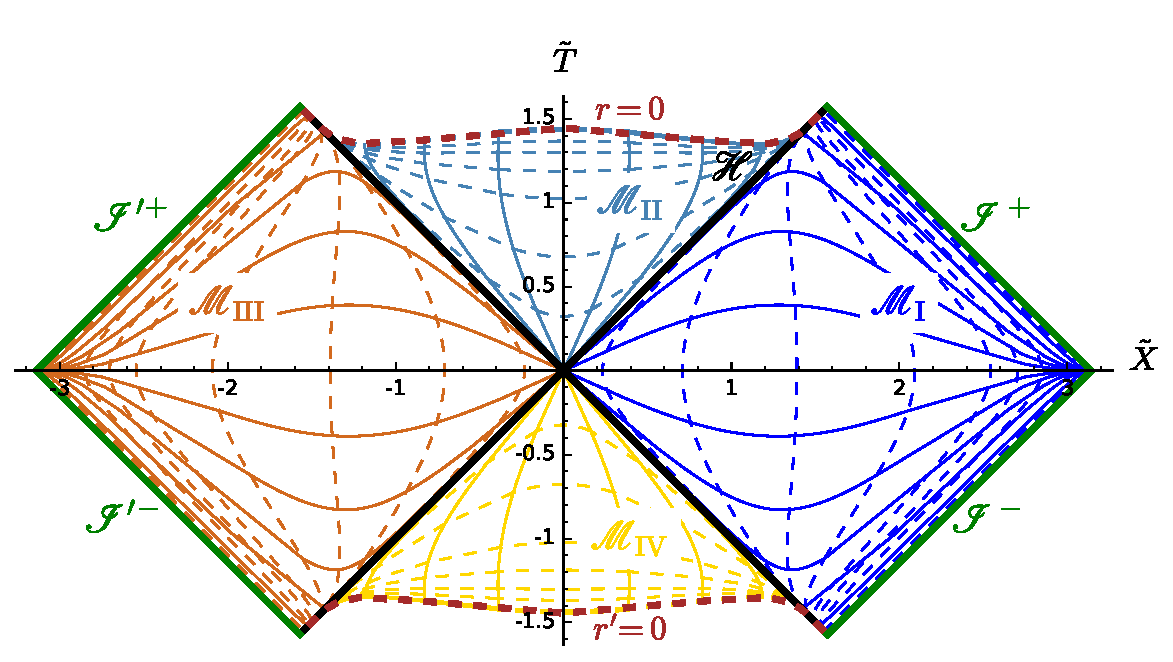
\includegraphics[width=0.9\textwidth]{max_carter-penrose-FN.pdf}}
\caption[]{\label{f:max:carter-penrose-FN} \footnotesize
Carter-Penrose diagram of the Schwarzschild spacetime based on the Frolov-Novikov coordinates.
Solid curves denote the same hypersurfaces of constant Schwarzschild-Droste coordinate
$t$ as in Fig.~\ref{f:max:carter-penrose-std}: in region $\M_{\rm I}$, from the $\hat{X}$-axis to the top: $t=0$, $2m$,
$5m$, $10m$, $20m$ and $50m$;
in region $\M_{\rm II}$, from the $\hat{T}$-axis
to the right: $t=0$, $2m$, $5m$, $10m$, $20m$ and $50m$,
Dashed curves denote the same hypersurfaces of constant Schwarzschild-Droste coordinate
$r$ as in Fig.~\ref{f:max:carter-penrose-std}: in region $\M_{\rm I}$, from the left to the right: $r=2.01m$, $2.1m$, $2.5m$, $4m$, $8m$, $12m$, $20m$ and $100m$;
in region $\M_{\rm II}$, from the bottom to the top: $r=1.98m$, $1.9m$, $1.7m$,
$1.5m$, $1.25m$, $m$, $0.5m$ and $0.1m$.
The color code
is the same as in Figs.~\ref{f:sch:kruskal_diag} and \ref{f:max:carter-penrose-std}.
Contrary to the Carter-Penrose of Fig.~\ref{f:max:carter-penrose-std}, this one is
associated to a regular conformal completion at null infinity of Schwarzschild spacetime. See Sec.~\ref{s:sam:reg_Carter-Penrose} for the
SageManifolds worksheet generating this figure.}
\end{figure}



To depict $\tilde{\M}$, let us introduce ``time+space'' coordinates
$(\tilde{T},\tilde{X})$,
which are related to $(\hat{U},\hat{V})$ in exactly the same way
as $(\hat{T},\hat{X})$ are related to $(\hat{U},\hat{V})$
[cf. Eq.~(\ref{e:max:hThX_hUhV})]:
\be \label{e:max:tTtX_tUtV}
    \left\{ \begin{array}{l}
    \tilde{T} = \tilde{U} + \tilde{V} \\
    \tilde{X} = \tilde{V} - \tilde{U}
    \end{array} \right.
    \iff
    \left\{ \begin{array}{l}
    \tilde{U} = \frac{1}{2} (\tilde{T} - \tilde{X}) \\[1ex]
    \tilde{V} = \frac{1}{2} (\tilde{T} + \tilde{X}) .
    \end{array} \right.
\ee
The range of $(\tilde{T},\tilde{X})$ is deduced from (\ref{e:max:range_tUtV}):
\bea
    \M:& &  -\pi < \tilde{T} - \tilde{X} <\pi,\quad
    -\pi < \tilde{T} + \tilde{X} < \pi \nonumber \\
    & &  \sinh[\tan((\tilde{T}-\tilde{X})/2)]
        \; \sinh[\tan((\tilde{T}+\tilde{X})/2)] < 1 . \label{e:max:range_tTtX}
\eea
The picture of $(\M,\w{g})$ in the $(\tilde{T},\tilde{X})$ plane is shown in
Fig.~\ref{f:max:carter-penrose-FN}. We shall call it a
\defin{regular Carter-Penrose diagram}\index{Carter-Penrose diagram!regular --}
of Schwarzschild spacetime.
As the singular Carter-Penrose diagram of Fig.~\ref{f:max:carter-penrose-std},
it has the property
to display the radial null geodesics as straight lines with slope $\pm 45^\circ$,
since $\tilde{U}$ (resp. $\tilde{V}$) is a function of $U$ only
(resp. $V$ only) [cf. Eq.~(\ref{e:max:def_tUtV})].
In particular, the bifurcate Killing horizon and the Schwarzschild horizon
are defined by:
\begin{subequations}
\begin{align}
    \hat{\Hor}:\quad&  \tilde{U} = 0 \quad\mbox{or}\quad \tilde{V} = 0 \ \iff \
    \tilde{T} = \tilde{X} \quad\mbox{or}\quad \tilde{T} = - \tilde{X} \\
    \Hor:\quad &  \tilde{U} = 0 \quad\mbox{and}\quad \tilde{V} > 0 \ \iff \
      \tilde{T} = \tilde{X} \quad\mbox{and}\quad \tilde{T} > 0 .
\end{align}
\end{subequations}
These relations follow immediately from (\ref{e:max:Hor_U_V}),
(\ref{e:max:def_tUtV}) and (\ref{e:max:tTtX_tUtV}).


At first sight, the main difference with the ``standard'' Carter-Penrose diagram
of Fig.~\ref{f:max:carter-penrose-std} is the more complicated shape of
the boundary around the $\tilde{T}$-axis. This follows from the third
condition in (\ref{e:max:range_tTtX}), which is more involved than
the third condition in (\ref{e:max:range_hThX}).
Actually this boundary corresponds to the curvature singularity limit $r\rightarrow 0$
or $r'\rightarrow 0$. Indeed, from Eq.~(\ref{e:max:r_UV}), we have
\be \label{e:max:r_zero_UV}
    r = 0 \iff UV = 1 .
\ee
In terms of the coordinates $(\hat{U},\hat{V})$, we have then
[cf. Eq.~(\ref{e:max:def_hUhV})]
\bea
    r = 0 &\iff & \tan \hat{U} \tan \hat{V} = 1 \iff \sin \hat{U} \cos \hat{V} =
    \cos\hat{U} \cos\hat{V} \nonumber \\
    &\iff & \cos\hat{U} \cos\hat{V} - \sin \hat{U} \cos \hat{V} = 0
     \iff \cos(\hat{U} + \hat{V}) = 0
     \iff \hat{U} + \hat{V} = \pm \frac{\pi}{2} .  \nonumber
\eea
Since $\hat{T} = \hat{U} + \hat{V}$, we get the simple relation
\be
    r = 0 \iff \hat{T} =  \pm \frac{\pi}{2} .
\ee
On the contrary, in terms of the coordinates $(\tilde{U},\tilde{V})$,
Eq.~(\ref{e:max:r_zero_UV}) becomes [cf.
Eq.~(\ref{e:max:def_tUtV})]
\[
    r = 0 \iff \sinh(\tan \tilde{U}) \sinh(\tan \tilde{V}) = 1 ,
\]
which yields to the complicated formula
\be \label{e:max:r_zero_tTtX}
    r = 0 \iff  \sinh[\tan((\tilde{T}-\tilde{X})/2)]
        \; \sinh[\tan((\tilde{T}+\tilde{X})/2)] = 1 .
\ee
This explains the more complex boundary of Fig.~\ref{f:max:carter-penrose-FN}
diagram with respect to Fig.~\ref{f:max:carter-penrose-std} diagram.

\begin{remark}
The shape of the Carter-Penrose diagram in Frolov \& Novikov's book (Fig.~5.2 of
Ref.~\cite{FroloN98}; see also Fig.~10.6 of Ref.~\cite{FroloZ11}) differs slightly from the diagram obtained here (Fig.~\ref{f:max:carter-penrose-FN}). This is because
the coordinates used by Frolov \& Novikov are constructed from the
Szekeres' version (up to a factor 2) of Kruskal-Szekeres coordinates:
$T' = T/\sqrt{e}$ and $X'=X/\sqrt{e}$
(cf. the historical note on p.~\pageref{n:max:KS_coord}).
Accordingly, in Frolov \& Novikov's version, one shall replace the $1$
in the right-hand side of Eq.~(\ref{e:max:r_zero_tTtX}) by $1/e$, yielding to
a different shape of the boundary $r=0$.
\end{remark}

\begin{remark}
As noticed by Frolov and Novikov \cite{FroloN98} (see their Sec.~5.1.3),
one can perform some
coordinate transformation from $(\tilde{U},\tilde{V})$ to get a
Carter-Penrose diagram with a straight line for the boundary $r=0$.
\end{remark}

Besides the shape of the boundary $r=0$, another difference between
the Carter-Penrose diagram based on Frolov-Novikov coordinates
(Fig.~\ref{f:max:carter-penrose-FN}) and the ``standard'' diagram
of Fig.~\ref{f:max:carter-penrose-std} is that the $t=\mathrm{const}$
hypersurfaces of the former (solid curves in Fig.~\ref{f:max:carter-penrose-FN})
are all tangent to the horizontal axis when $\tilde{X}\rightarrow \pm\pi$.
On the contrary, the same hypersurfaces in Fig.~\ref{f:max:carter-penrose-std}
reach the point $(\hat{T},\hat{X}) = (0,\pm\pi)$ with a finite slope.
We note that in this respect, the Carter-Penrose diagram of
Fig.~\ref{f:max:carter-penrose-FN} is similar to the conformal diagram of
Minkowski spacetime, as shown in Fig.~\ref{f:glo:conf_diag_Mink}, and
therefore display correctly the asymptotic flatness structure.
The failure of diagram of Fig.~\ref{f:max:carter-penrose-std} to reproduce
this behavior reflects the fact that the coordinates $(\hat{T},\hat{X})$ are singular on the
boundary, as discussed in Sec.~\ref{s:max:discus_hUhV}.

\begin{figure}
\centerline{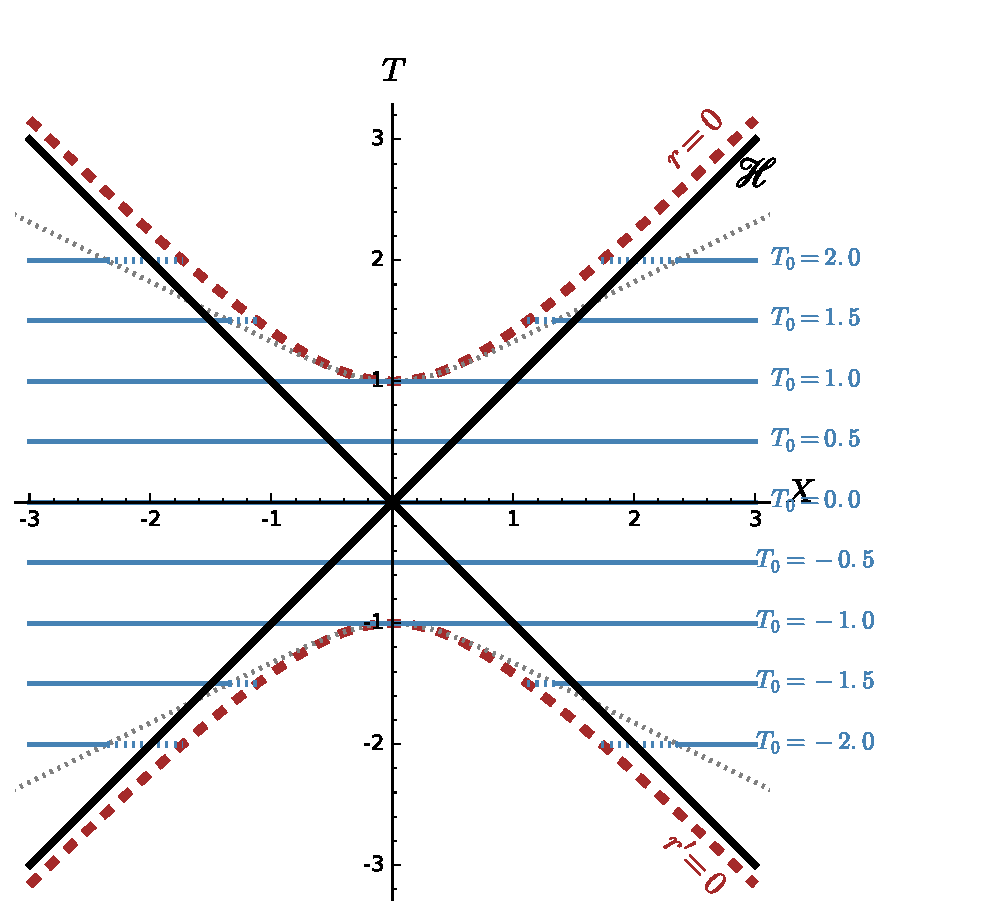
\includegraphics[width=0.6\textwidth]{max_constant_T_slices.pdf}}
\caption[]{\label{f:max:constant_T_slices} \footnotesize
Kruskal diagram with the hypersurfaces $\Sigma_{T_0}$ (defined by $T=T_0 = \mathrm{const.}$) as blue horizontal lines. For $|T_0|>1$, the dotted part of
$\Sigma_{T_0}$ corresponds to a region that cannot be embedded isometrically in
the Euclidean space. When $T_0$ varies, the limit of these regions form
the grey dotted curve.}
\end{figure}

%%%%%%%%%%%%%%%%%%%%%%%%%%%%%%%%%%%%%%%%%%%%%%%%%%%%%%%%%%%%%%%%%%%%%%%%%%%%%%%%%%%%%

\section{Einstein-Rosen bridge}

\subsection{Hypersurfaces of constant Kruskal-Szekeres time} \label{s:max:hyp_const_T}

To get some insight on the maximally extended Schwarzschild
spacetime $(\M,\w{g})$, let us examine the geometry of a slice of constant
Kruskal-Szekeres time $T$, i.e. a hypersurface $\Sigma_{T_0}$ defined
in terms of the global Kruskal-Szekeres coordinates $(T,X,\th,\ph)$ by
$T=T_0$, where $T_0\in\mathbb{R}$ is a constant
(cf. Fig.~\ref{f:max:constant_T_slices}).
The 3-uple $(x^i)=(X,\th,\ph)$ is then a coordinate system on $\Sigma_{T_0}$
subject to the constraint expressed in (\ref{e:sch:def_M_extend}):
\be
    X^2 > T_0^2 - 1 .
\ee
Consequently
\begin{itemize}
\item if $|T_0|< 1$, the hypersurface $\Sigma_{T_0}$ is connected
and diffeomorphic to $\R\times\SS^2$, the coordinate $X$ spanning $\R$ and
$(\th,\ph)$ spanning $\SS^2$.
\item if $|T_0| \geq 1$, $\Sigma_{T_0}$ has two connected components,
defined by
$X < - \sqrt{T_0^2 - 1}$ and $X > \sqrt{T_0^2 - 1}$ respectively
(cf. Fig.~\ref{f:max:constant_T_slices}).
Each of them is diffeomorphic to $\R\times\SS^2$.
\end{itemize}
For future convenience, we split $\Sigma_{T_0}$ in two disjoint parts, according
to the sign of $X$:
\be
    \Sigma^+_{T_0} = \left\{ p \in \Sigma_{T_0},\quad X(p) \geq 0 \right\}
    \quad\mbox{and}\quad
    \Sigma^-_{T_0} = \left\{ p \in \Sigma_{T_0},\quad X(p) < 0 \right\} .
\ee
For $|T_0|< 1$, there is a slight asymmetry between the
two parts: $\Sigma^+_{T_0}$ is a manifold with boundary
(cf. Sec.~\ref{s:bas:manif_boundary}), the boundary corresponding
to $X=0$, while $\Sigma^-_{T_0}$ is not.
For $|T_0|\geq 1$, $\Sigma^+_{T_0}$ and $\Sigma^-_{T_0}$ are nothing but the
two connected components of $\Sigma_{T_0}$.

The geometry of $\Sigma_{T_0}$ is defined by the metric $\w{\gamma}$
induced on it by $\w{g}$:
\be \label{e:max:gam_induced}
    \gamma_{ij} \D x^i \D x^j =
    \frac{32 m^3}{r} \, \mathrm{e}^{-r/2m} \,  \D X^2
     +  r^2 \left( \D\th^2 + \sin^2\th\, \D\ph^2 \right) ,
\ee
where $r$ is the function of $X$ defined by
\be \label{e:max:Sigma0_r_X}
    r = r(X) = 2 m  \tilde{W}_0(X^2 - T_0^2) .
\ee
The line element (\ref{e:max:gam_induced}) is obtained by setting $T=T_0$ and
$\D T = 0$ in (\ref{e:sch:metric_KS_TX}).
Since $r>0$, the metric (\ref{e:max:gam_induced}) is clearly positive definite,
i.e. $\w{\gamma}$ is a Riemannian metric and $\Sigma_{T_0}$ is a
spacelike hypersurface.

The graph of the function $r(X)$ is shown in Fig.~\ref{f:max:SigmaT0_r_X}.
Once restricted to positive (resp. negative) values of $X$, this function is a bijection
$(X_0, +\infty)\rightarrow (r_0, +\infty)$ (resp. $(-\infty, -X_0)\rightarrow (r_0, +\infty)$), where
\be \label{e:max:def_X0_r0}
    X_0 = \left\{ \begin{array}{ll}
        0 & \ \mbox{if}\quad  |T_0| < 1 \\
        \sqrt{T_0^2-1} & \ \mbox{if}\quad  |T_0| \geq 1.
        \end{array} \right.
    \quad \mbox{and}\quad
    r_0 = \left\{ \begin{array}{ll}
        2m \tilde{W}_0(-T_0^2) & \ \mbox{if}\quad  |T_0| < 1 \\
        0 & \ \mbox{if}\quad  |T_0| \geq 1.
        \end{array} \right.
\ee
The inverse of this bijection is\footnote{Let us recall that
$\tilde{W}_0^{-1}(x) = \mathrm{e}^x (x-1)$.}
\be \label{e:max:Sigma0_X_r}
    X = X(r) = \pm \sqrt{\mathrm{e}^{r/2m} \left( \frac{r}{2m} - 1 \right) + T_0^2} ,
\ee
with the $+$ sign on $\Sigma^+_{T_0}$ and the $-$ sign
on $\Sigma^-_{T_0}$.

\begin{figure}
\centerline{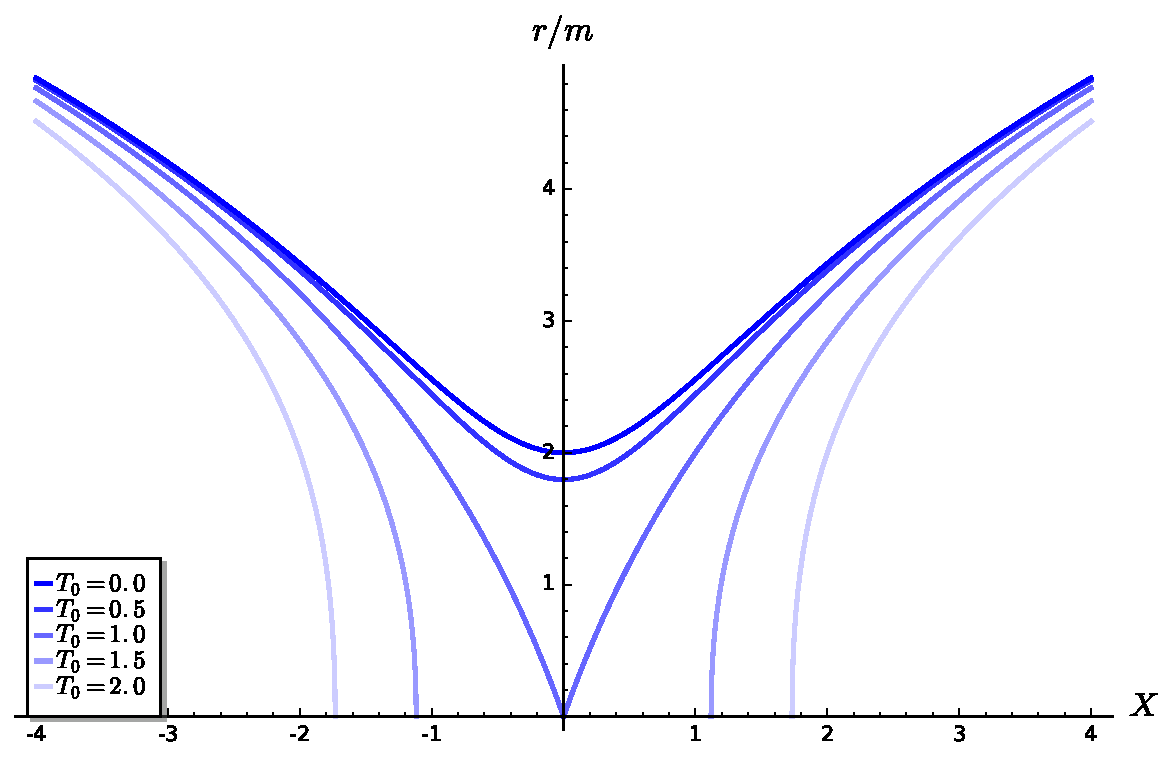
\includegraphics[height=0.35\textheight]{max_SigmaT0_r_X.pdf}}
\caption[]{\label{f:max:SigmaT0_r_X} \footnotesize
Function $r = r(X)$ on the hypersurface $\Sigma_{T_0}$, for the same values
of $T_0$ as in Fig.~\ref{f:max:constant_T_slices}.}
\end{figure}

We may use the above bijection to introduce coordinates $(r,\th,\ph)$ instead of $(X,\th,\ph)$
on each of the two regions $\Sigma^+_{T_0}$ and $\Sigma^-_{T_0}$.
Differentiating (\ref{e:max:Sigma0_X_r}) leads to
\[
    \D X = \pm \frac{r \mathrm{e}^{r/2m}}{8m^2 \sqrt{\mathrm{e}^{r/2m} \left( \frac{r}{2m} - 1 \right) + T_0^2}} \, \D r .
\]
Substituting in (\ref{e:max:gam_induced}) we get the expression of the
metric on $\Sigma_{T_0}$ in terms of the coordinates $(x^i) = (r,\th,\ph)$:
\be \label{e:max:Sigma0_metric}
    \gamma_{ij}\,  \D x^i \D x^j = \left(
    1 - \frac{2m}{r} \left(1 -  T_0^2 \mathrm{e}^{-r/2m} \right) \right) ^{-1} \, \D r^2
     +  r^2 \left( \D\th^2 + \sin^2\th\, \D\ph^2 \right) .
\ee
\begin{remark} \label{r:max:check_metric_SigmaT0}
As a check of the above formula, we notice that for $T_0=0$ it reduces to the
metric of a slice $t=\mathrm{const}$ in Schwarzschild-Droste coordinates
[set $\D t =0$ in Eq.~(\ref{e:sch:Schwarz_metric_SD})]. This is correct since
the positive-$X$ half of the hypersurface $T=0$ in Kruskal-Szekeres coordinates,
i.e. $\Sigma_0^+$,
coincides with the hypersurface $t=0$ in Schwarzschild-Droste coordinates,
as it can be seen by setting $T=0$ in Eq.~(\ref{e:sch:KS_SD_I})
(see also Fig.~\ref{f:max:constant_T_slices}).
\end{remark}

\subsection{Isometric embedding in 3-dimensional Euclidean space}

We may visualize the geometry of the spacelike hypersurface $\Sigma_{T_0}$
via some isometric embedding of some 2-dimensional slice of it
in the 3-dimensional Euclidean space $(\R^3, \w{f})$, $\w{f}$ being the standard
flat (Euclidean) metric.
By \defin{isometric embedding}\index{isometric!embedding}\index{embedding!isometric --}
of a 2-dimensional Riemannian manifold $(\Sp,\w{g})$
in $(\R^3,\w{f})$, it is meant a \emph{smooth embedding} $\Phi:\ \Sp \rightarrow \R^3$,
as defined in Sec.~\ref{s:bas:embed},
such that the metric induced on $\Phi(\Sp)$ by the Euclidean metric of $\R^3$
coincides with the original metric $\w{g}$ on $\Sp$:
\be \label{e:max:isometric_emb}
    \forall p\in \Sp,\quad  \forall (\w{u},\w{v})\in (T_p \Sp)^2,\quad
        \w{f}(\Phi^*(\w{u}), \Phi^*(\w{v})) = \w{g}(\w{u},\w{v}) ,
\ee
where $\Phi^*(\w{u})$ is the ``image of the vector $\w{u}$ by $\Phi$'', i.e.
the pushforward of $\w{u}$ by $\Phi$, as defined in
Sec.~\ref{s:bas:Lie_der_vector}. Another phrasing of the
isometry property (\ref{e:max:isometric_emb}) is: the pullback of $\w{f}$
on $\Sp$ by $\Phi$ coincides with $\w{g}$: $\Phi^*\w{f} = \w{g}$ [cf. Eq.~(\ref{e:bas:def_pullback})].

Taking into account the spherical symmetry
of $\Sigma_{T_0}$, there is no loss of generality in choosing the
equatorial plane $\theta=\pi/2$ as the 2-dimensional slice. We shall denote
it by $\Sigma_{T_0}^{\rm eq}$.
Coordinates on $\Sigma_{T_0}^{\rm eq}$ are $(x^a)=(X,\ph)$, or
on each of the two parts $\Sigma_{T_0}^{+,\rm eq}$ ($X\geq 0$) and
$\Sigma_{T_0}^{-,\rm eq}$ ($X<0$),
$(x^a)=(r,\ph)$.
If $|T_0| < 1$, the topology of $\Sigma_{T_0}^{\rm eq}$ is
$\R\times\SS^1$, i.e. that of a cylinder, while for $|T_0| \geq 1$, it has
two connected components, $\Sigma_{T_0}^{+,\rm eq}$ and
$\Sigma_{T_0}^{-,\rm eq}$, each of them having the topology of a cylinder.

The metric induced by $\w{g}$
on $\Sigma_{T_0}^{\rm eq}$,
$\w{q}$ say, is obtained by setting $\th=\pi/2$ and $\D\th=0$ in
Eq.~(\ref{e:max:Sigma0_metric}):
\be \label{e:max:metric_q}
    q_{ab}\,  \D x^a \D x^b = \left(
    1 - \frac{2m}{r} \left(1 -  T_0^2 \mathrm{e}^{-r/2m} \right) \right) ^{-1}
     \, \D r^2 +  r^2 \D\ph^2 .
\ee
Given the invariance in $\ph$, it is
quite natural to embed $(\Sigma_{T_0}^{\rm eq},\w{q})$ as
a surface of revolution in the Euclidean space $(\R^3, \w{f})$.
Describing $\R^3$ with cylindrical coordinates $(x^i) = (r,z,\ph)$,
the Euclidean metric $\w{f}$ is
\be
    f_{ij}\,  \D x^i \D x^j = \D r^2 + \D z^2 + r^2 \D\ph^2 .
\ee
A surface of revolution $\Sp$ in $\R^3$ is described by an equation of the type
$z = Z(r)$. On such a surface, one has therefore
$\D z = Z'(r) \, \D r$, so that the metric $\w{h}$ induced by $\w{f}$ on it is
\be \label{e:max:metric_h}
    h_{ab}\,  \D x^a \D x^b = \left( 1 + Z'(r)^2 \right) \D r^2
            + r^2 \D\ph^2 .
\ee
Comparing (\ref{e:max:metric_h}) with (\ref{e:max:metric_q}),
we see that a possible isometric embedding of $\Sigma_{T_0}^{\rm eq}$ into $\R^3$
is
\be \label{e:max:def_embedding_Phi}
    \begin{array}{clcl}
    \Phi: & \Sigma_{T_0}^{\rm eq} & \longrightarrow & \R^3 \\
        & (X,\ph) & \longmapsto & (r,z,\ph) = \left(r(X), \pm Z(r(X)), \ph \right) ,
    \end{array}
\ee
with (i) the sign $\pm$ being $+$ on $\Sigma_{T_0}^{+,\rm eq}$ and $-$ on
$\Sigma_{T_0}^{-,\rm eq}$ and (ii) the function $Z$ obeying
\[
   1 + Z'(r)^2 =  \left(
    1 - \frac{2m}{r} \left(1 -  T_0^2 \mathrm{e}^{-r/2m} \right) \right) ^{-1} .
\]
Thanks to Eq.~(\ref{e:max:Sigma0_X_r}), this expression can be recast as
\be \label{e:max:Zp2}
    Z'(r)^2 = \frac{1 - T_0^2  \mathrm{e}^{-r/2m}}{
    T_0^2  \mathrm{e}^{-r/2m} + \frac{r}{2m} - 1} =
    \frac{\mathrm{e}^{r/2m} - T_0^2}{X(r)^2} .
\ee
For $|T_0|<1$, i.e. when $\Sigma_{T_0}^{\rm eq}$ is connected, the
map (\ref{e:max:def_embedding_Phi}) defines a smooth embedding if, and only
if, at the boundary $X=0$ between $\Sigma_{T_0}^{+,\rm eq}$ and
$\Sigma_{T_0}^{-,\rm eq}$, the following holds:
\be
    Z(r(0)) = 0 \quad\mbox{and}\quad Z'(r(0)) = \infty .
\ee
The condition $Z(r(0)) = 0$ insures the continuity of the embedded surface
$\Phi(\Sigma_{T_0}^{\rm eq})$,
while $Z'(r(0)) = +\infty$ insures that it has a vertical tangent at
the junction between $\Phi(\Sigma_{T_0}^{+,\rm eq})$ and
$\Phi(\Sigma_{T_0}^{-,\rm eq})$, so that it is
a smooth surface. Fortunately, the condition $Z'(r(0)) = \infty$
is automatically fulfilled from the second expression of
$Z'(r)^2$ in (\ref{e:max:Zp2}): $Z'(r)^2$ clearly diverges at $X=0$.
Moreover, in order for the isometric embedding $\Phi$ to be well defined, the right-hand side
of (\ref{e:max:Zp2}) must be non-negative. Since the denominator of the last
term is manifestly non-negative, the sign is determined by the numerator. Hence
the condition $\mathrm{e}^{r/2m} \geq T_0^2$, or equivalently,
\be \label{e:max:cond_r_embed}
    r \geq 4 m \ln |T_0| .
\ee
For $|T_0|\leq 1$, this condition is always fulfilled, since $\ln |T_0| \leq 0$
and $r \geq 0$. For $|T_0| > 1$, it implies the existence of a minimal value
of $r$,
\be \label{e:max:r_emb}
    r_{\rm emb}(T_0) :=  4 m \ln |T_0|,
\ee
such that the part of $\Sigma_{T_0}^{\rm eq}$ with $r< r_{\rm emb}(T_0)$
cannot be embedded isometrically in the Euclidean 3-space.
\begin{remark}
The above result should not be surprising since there is
no guarantee that a 2-dimensional Riemannian manifold can
be isometrically embedded in the 3-dimensional Euclidean space.
The relevant theorem here is \emph{Nash embedding theorem}\index{Nash embedding theorem}\index{embedding!Nash -- theorem} \cite{Nash56}, which
states that any smooth Riemannian manifold of dimension $n$ can be isometrically
embedded in the Euclidean space $(\R^m,\w{f})$, with $m \leq n(n+1)(3n+11)/2$.
For $n=2$, we get $m\leq 51$, so there is really no guarantee that $m=3$
is sufficient...
\end{remark}

Via (\ref{e:max:Sigma0_r_X}) and the fact that the rescaled Lambert function
$\tilde{W}_0$ is an increasing function (cf. Fig.~\ref{f:max:lambert_rescaled}), of inverse $F(x)=\mathrm{e}^x(x-1)$,
the condition (\ref{e:max:cond_r_embed}) can be turned into a condition
on $X$:
\be
    |X| \geq X_{\rm emb}(T_0) := |T_0| \sqrt{2\ln |T_0|} .
\ee
This limit is shown as the grey dotted curve in Fig.~\ref{f:max:constant_T_slices}.

\begin{figure}
\centerline{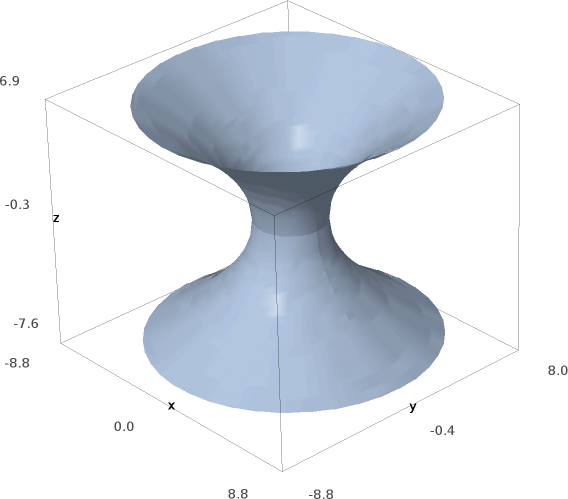
\includegraphics[height=0.4\textheight]{max_flamm_paraboloid.png}}
\caption[]{\label{f:max:flamm_paraboloid} \footnotesize
Flamm paraboloid\index{Flamm paraboloid}: isometric embedding in the Euclidean $\R^3$
of the spacelike slice $T=0$ and $\th=\pi/2$ of Schwarzschild spacetime.
The $(x,y)$ coordinates are the standard Cartesian coordinates of $\R^3$ related
to $(r,\ph)$ via $x=r\cos\ph$ and $y=r\sin\ph$. The labels are in units of $m$.}
\end{figure}

Summarizing, the minimal value of $r$ on the embedded surface is
$r_0$ [cf. Eq.~(\ref{e:max:def_X0_r0})] for $|T_0|\leq 1$ or
$r_{\rm emb}(T_0)$ for $|T_0| > 1$:
\be
    r_{\rm min}(T_0) = \left\{ \begin{array}{ll}
        2m \tilde{W}_0(-T_0^2) & \ \mbox{if}\quad  |T_0| \leq 1 \\
        4 m \ln |T_0| & \ \mbox{if}\quad  |T_0| > 1.
        \end{array} \right.
\ee
Note that $r_{\rm min}(T_0)$ is a continuous function, with the peculiar values $r_{\rm min}(0) = 2m$ and $r_{\rm min}(1) = 0$.
The embedding function $Z(r)$ is found by integration of $Z'(r)$, as given
by (\ref{e:max:Zp2}), from $r_{\rm min}(T_0)$ to $r$:
\be \label{e:max:Z_r_integral}
    Z(r) = 2m \int_{\frac{\scriptstyle r_{\rm min}(T_0)}{\scriptstyle 2m}}^{\frac{\scriptstyle r}{\scriptstyle 2m}}
        \sqrt{ \frac{1 - T_0^2 \mathrm{e}^{-x}}{ T_0^2 \mathrm{e}^{-x} + x - 1}}
        \, \D x .
\ee
The integral cannot be computed exactly in terms of elementary functions, except for
$T_0 = 0$, where it reduces to
\[
    Z(r) = 2 m \int_1^{\frac{\scriptstyle r}{\scriptstyle 2m}}
        \frac{\D x}{\sqrt{x-1}}  \qquad (T_0=0) .
\]
Hence
\be \label{e:max:Z_r_Flamm}
    \encadre{ Z(r) = 4 m \sqrt{\frac{r}{2m} - 1 }} \qquad (T_0=0).
\ee
According to (\ref{e:max:def_embedding_Phi}), the whole surface
$\Phi(\Sigma_{T_0}^{\rm eq})$ is obtained by considering $z = -Z(r)$ as well.
The surface equation in terms of the cylindrical coordinates $(r,z,,\ph)$
of $\R^3$ is then $z^2 = 16m^2(r/2m-1)$, or
\be \label{e:max:z2_r_Flamm}
    \encadre{ z^2 = 8 m (r - 2m) }.
\ee
We recognize the equation of a parboloid of revolution around the $z$-axis.
It is known as \defin{Flamm paraboloid}\index{Flamm paraboloid} \cite{Flamm1916} and is depicted in Fig.~\ref{f:max:flamm_paraboloid}. Its topology is clearly that of
a cylinder ($\R\times\SS^1$). The geometry is different though: from top
to bottom, the radius of the ``cylinder'' decreases to a minimal value, $r_{\rm min}=2m$,
and then increases. The ``neck'' around $r=r_{\rm min}$, or equivalently $X=0$, is called the
\defin{Einstein-Rosen bridge}\index{Einstein-Rosen bridge} \cite{EinstR35}.
Contemplating the slice $T=0$ in the
Kruskal diagram of Fig.~\ref{f:max:constant_T_slices}, we realize that
this ``bridge'' connects the two asymptotically flat regions $\M_{\rm I}$ and
$\M_{\rm III}$. The Einstein-Rosen bridge is also called
the \defin{Schwarzschild wormhole}\index{Schwarzschild!wormhole}\index{wormhole!Schwarzschild --}. However, it is not
a \emph{traversable}\index{traversable!wormhole}\index{wormhole!traversable --} wormhole: it is clear from the Kruskal diagram
(Figs.~\ref{f:sch:kruskal_diag} and \ref{f:max:constant_T_slices})
or the Carter-Penrose diagram (Fig.~\ref{f:max:carter-penrose-FN}) that no
timelike or null worldline can go from $\M_{\rm I}$ to
$\M_{\rm III}$.

\begin{figure}
\begin{center}
\begin{tabular}{ccc}
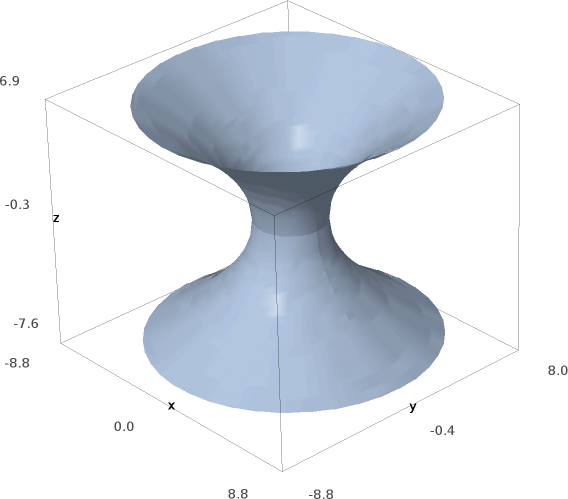
\includegraphics[width=0.33\textwidth]{max_flamm_paraboloid.png} &
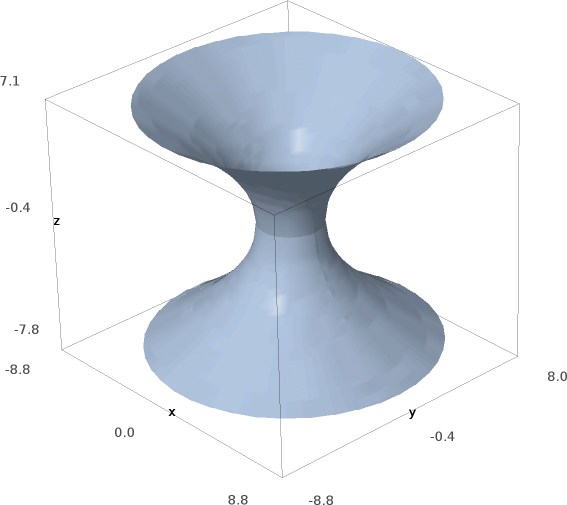
\includegraphics[width=0.33\textwidth]{max_embedding_T0_05.png} &
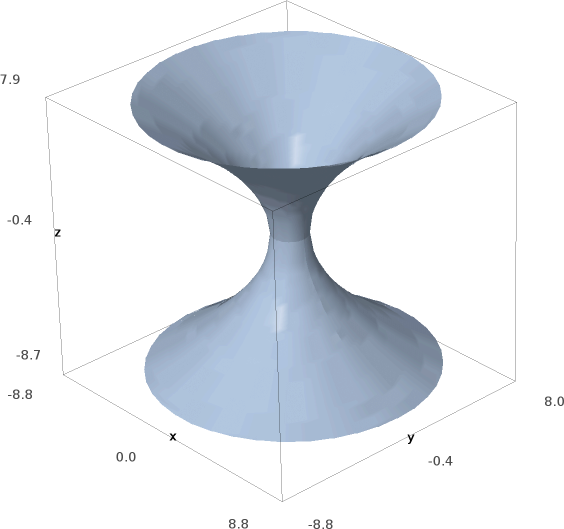
\includegraphics[width=0.33\textwidth]{max_embedding_T0_09.png} \\
$T_0=0$ & $T_0=0.5$ & $T_0=0.9$
\end{tabular} \\
\begin{tabular}{ccc}
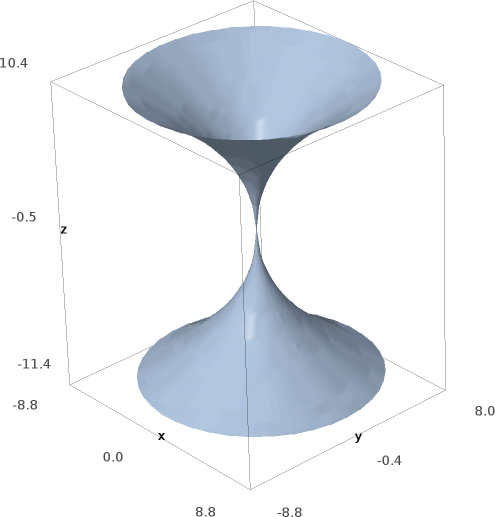
\includegraphics[width=0.33\textwidth]{max_embedding_T0_10.png} &
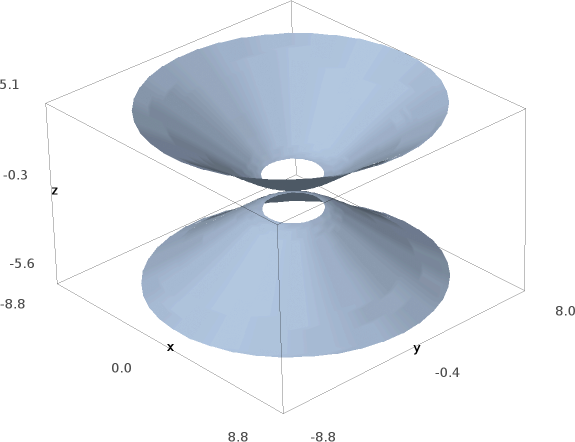
\includegraphics[width=0.33\textwidth]{max_embedding_T0_15.png} &
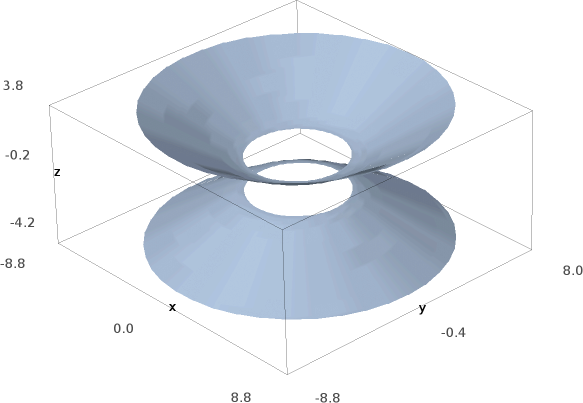
\includegraphics[width=0.33\textwidth]{max_embedding_T0_20.png} \\
$T_0=1$ & $T_0=1.5$ & $T_0=2$
\end{tabular}
\end{center}
\caption[]{\label{f:max:embeddings} \footnotesize
Sequence of isometric embeddings in the Euclidean space
of spacelike slices of Schwarzschild spacetime defined by
$T=T_0$ and $\th=\pi/2$. The slices are those shown in the Kruskal diagram
of Fig.~\ref{f:max:constant_T_slices} (except for $T_0=0.9$).
The first embedding ($T_0=0$) is the
Flamm paraboloid depicted in Fig.~\ref{f:max:flamm_paraboloid}.
In the disconnected case ($T_0=1.5$ and $T_0=2.0$),
the distance
between the upper and lower parts is arbitrary (chosen here to be $\Delta z = 1$).}
\end{figure}

When $T_0\not=0$, the integral in (\ref{e:max:Z_r_integral}) has to
be computed numerically (see Sec.~\ref{s:sam:Einstein-Rosen} for the computation with SageMath).
The resulting embedded surfaces $\Phi(\Sigma_{T_0}^{\rm eq})$ are shown in
Fig.~\ref{f:max:embeddings} for the values of $T_0$ involved in the
Kruskal diagram of Fig.~\ref{f:max:constant_T_slices}.
When $T_0$ increases from $0$, the ``neck'' becomes thiner and thiner.
At $T_0=1$, it ceases to be connected. As mentionned above, for $T_0 > 1$,
the surface $\Sigma_{T_0}^{\rm eq}$ can no longer be entirely
isometrically embedded in the Euclidean 3-space. Hence the holes in the central
parts of the surfaces for $T_0=1.5$ and $T_0=2$. These holes correspond
to the dotted segments in Fig.~\ref{f:max:constant_T_slices} and their radii
are given by Eq.~(\ref{e:max:r_emb}). Note that the tangents to the
embedded surfaces at their inner boundaries are horizontal.

The evolution of $\Sigma_{T_0}$ as $T_0$ increases is not surprising if one
remembers that the Kruskal-Szekeres time coordinate $T$ is not associated
with any timelike Killing vector of Schwarzschild spacetime.
The sequence shown in Fig.~\ref{f:max:embeddings} can be thought of as
representing the dynamics of the Schwarzschild wormhole, in particular
its ``pinching-off'' at $T_0=1$, which forbids any traveler to go through it.

\begin{remark}
We have restricted ourselves to slices $T=\mathrm{const.}$ of Schwarzschild
spacetime, with the isometric embedding limitation for $|T|>1$. We refer the
reader to Ref.~\cite{CollaK12} for more general slices and the corresponding
embedding diagrams.
\end{remark}

\begin{figure}
\centerline{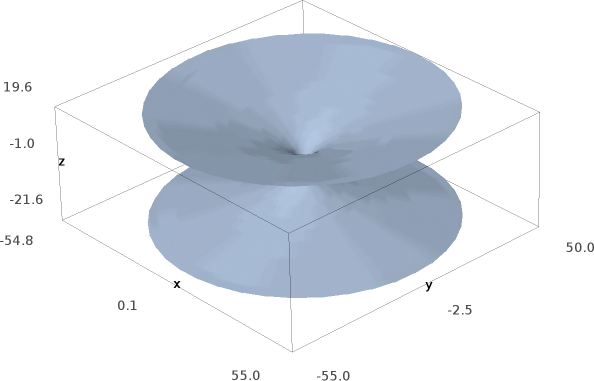
\includegraphics[height=0.3\textheight]{max_flamm_paraboloid_far.png}}
\caption[]{\label{f:max:flamm_paraboloid_far} \footnotesize
Same Flamm paraboloid\index{Flamm paraboloid} as in Fig.~\ref{f:max:flamm_paraboloid}
but seen from farther away. Despite being more and more flat, none of the two sheets
is asymptotic to a plane.}
\end{figure}

\begin{remark}
There are many inexact plots of embeddings of spatial sections
of Schwarz\-schild spacetime in the literature, including renown textbooks.
A first common error is to draw the two ends of the embedded surface as asymptotic to flat
planes, which a paraboloid is not (the vertical distance between the two ends grows
unbounded, as $\sqrt{r}$, cf. Eq.~(\ref{e:max:Z_r_Flamm}) and Fig.~\ref{f:max:flamm_paraboloid_far}).
This is correct from a topological point of view,
but not from the geometrical one, i.e. the embedding depicted in this way
is not an isometry. Probably this results from some confusion with asymptotic
flatness: it is true that the metric (\ref{e:max:metric_q}) tends
to a flat metric when $r\rightarrow +\infty$, reflecting the asymptotic
flatness of Schwarzschild spacetime, but the associated curvature does not
decay fast enough to allow the embedded surface to be tangent to a plane.
A second error regards the embeddings for $|T_0|> 1$, which
are depicted as variants of that $T_0=1$ (cf. Fig.~\ref{f:max:embeddings}),
with two spikes at $r=0$, simply pushed apart. However,
as discussed above, the isometric embeddings with $T=\mathrm{const}$
cannot reach the region near $r=0$ for $|T_0|> 1$.
\end{remark}

\begin{hist}
In 1916, very soon after the publication of Schwarzschild solution
\cite{Schwa1916}, the Austrian physicist Ludwig Flamm (1885-1964) showed that the slice $t=\mathrm{const}$
and $\th=\pi/2$ in Schwarzschild-Droste coordinates $(t,r,\th,\ph)$
can be isometrically embedded in the Euclidean space as a paraboloid of
revolution obeying Eq.~(\ref{e:max:z2_r_Flamm}) \cite{Flamm1916}.
Let us recall that the positive-$X$ part of the hypersurface $T=0$ considered here coincides with the
hypersurface $t=0$ (cf. Remark~\ref{r:max:check_metric_SigmaT0} on p.~\pageref{r:max:check_metric_SigmaT0}). Although he draw the whole paraboloid (actually
a parabola in a 2-dimensional plot --- Fig.~2 of Ref.~\cite{Flamm1916}), Flamm did not seem to have considered
the negative-$z$ part as physically relevant. In other words,
he limited his considerations to $\M_{\rm I}$ and did not contemplate any bridge to
the extension $\M_{\rm III}$.
\end{hist}

\subsection{Isotropic coordinates}

Let us consider a hypersurface of constant Schwarzschild-Droste time $t$
in $\M_{\rm I}$. According to Eq.~(\ref{e:max:TsX_tanh_t}), this hypersurface
obeys
\be \label{e:max:T_X_const_t}
    T = \tanh\left(\frac{t}{4m}\right) \, X,
\ee
with $X>0$,
which implies that it is represented by a straight half-line from the origin
in the Kruskal diagram (cf. Fig.~\ref{f:sch:kruskal_diag}).
Similarly, a hypersurface of constant $t'$
in $\M_{\rm III}$ obeys an equation identical to (\ref{e:max:T_X_const_t}),
except for $t$ replaced by $t'$ and $X<0$ [cf. Eq.~(\ref{e:sch:KS_SD_III})].
Accordingly, for $t'=t$, the union of these two hypersurfaces
forms a hypersurface of $\M$ ruled by Eq.~(\ref{e:max:T_X_const_t}),
with $X<0$ or $X>0$. If we add the points $(T,X)=(0,0)$ to it (i.e. the
bifurcation sphere $\Sp$ (cf. Sec.~\ref{s:max:bifur_Kill_hor}),
we obtain a connected hypersurface in which $X$ takes all values in
the range $(-\infty,+\infty)$. Let us call $\mathcal{S}_t$ this hypersurface.
In other words, $\mathcal{S}_t$ is the hypersurface of $\M$ defined by
Eq.~(\ref{e:max:T_X_const_t}) with $X\in\R$.
Note that for $t=0$, this hypersurface coincides with the hypersurface
$T=0$ introduced in Sec.~\ref{s:max:hyp_const_T}: $\mathcal{S}_0 = \Sigma_0$.
But for $t\not=0$, $\mathcal{S}_t \not= \Sigma_T$.

There are two Schwarzschild-Droste coordinate systems on $\mathcal{S}_t$:
$(r,\th,\ph)$ on $\mathcal{S}_t\cap \M_{\rm I}$ and $(r',\th,\ph)$ on
$\mathcal{S}_t\cap \M_{\rm III}$, with both $r$ and $r'$ ranging
$(2m,+\infty)$.
Let us introduce on $\mathcal{S}_t$ a third coordinate system $(x^i)=(\bar{r},\th,\ph)$
as follows:
\begin{subequations}
\begin{align}
& \mbox{on}\ \mathcal{S}_t\cap \M_{\rm I}:  & & \bar{r} \in \left(\frac{m}{2}, +\infty \right), & &
     r = \bar{r} \left( 1 + \frac{m}{2\bar{r}} \right)^2 \label{e:max:r_riso}\\
& & & & & \iff \bar{r} = \frac{1}{2} \left( r - m + \sqrt{r (r-2m)} \right) \\
&\mbox{on}\ \mathcal{S}_t\cap  \M_{\rm III}:& &
    \bar{r} \in \left(0, \frac{m}{2} \right), & &
    r' = \bar{r} \left( 1 + \frac{m}{2\bar{r}} \right)^2 \label{e:max:rp_riso} \\
& & & & & \iff \bar{r} = \frac{1}{2} \left( r' - m - \sqrt{r' (r'-2m)} \right) \\
&\mbox{on}\ \mathcal{S}_t\cap \Sp : & & \bar{r} = \frac{m}{2} .& &
\end{align}
\end{subequations}
The range of $\bar{r}$ is thus $(0,+\infty)$.
The graph of the function
$\bar{r} \mapsto \bar{r}(1+m/(2\bar{r}))^2$ is depicted in
Fig.~\ref{f:max:r_riso}. We can separate this graph in two parts:
$\bar{r}\in (0,m/2)$ (the $\M_{\rm III}$ part) and $\bar{r}\in (m/2, +\infty)$
(the $\M_{\rm I}$ part). In each of these part, there is a one-to-one
correspondance between $\bar{r}$ and $r$ (or $r'$). Note that
\begin{subequations}
\begin{align}
    & \mbox{when}\ r\rightarrow +\infty,\quad \bar{r} \sim r \\
    & \mbox{when}\ r'\rightarrow +\infty,\quad \bar{r} \sim \frac{m^2}{4 r'} .
\end{align}
\end{subequations}

\begin{figure}
\centerline{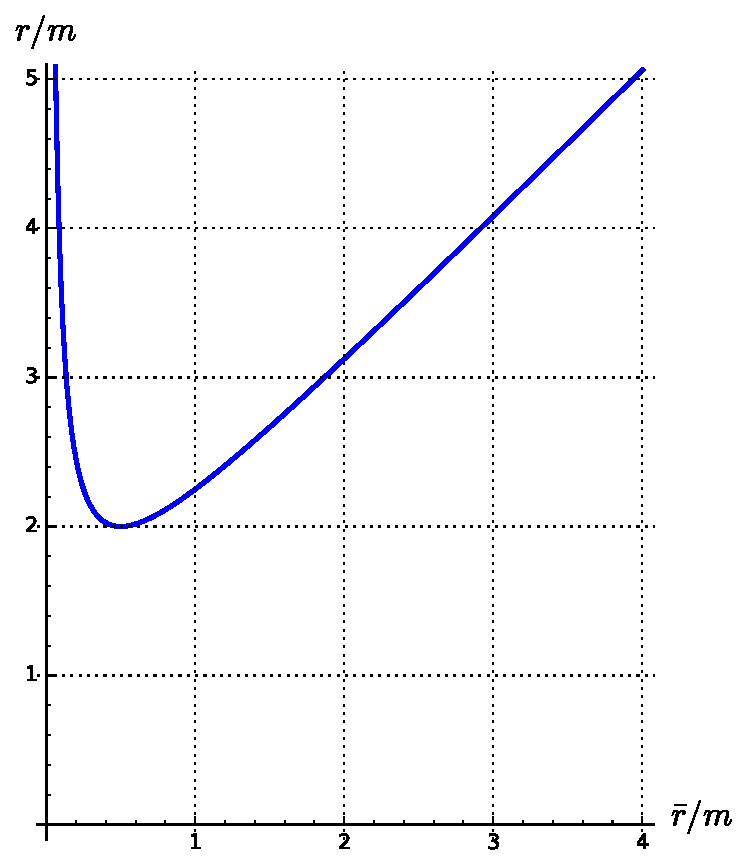
\includegraphics[height=0.4\textheight]{max_r_riso.pdf}}
\caption[]{\label{f:max:r_riso} \footnotesize
Areal radius $r$ as a function of the isotropic coordinate $\bar{r}$.}
\end{figure}

When $t$ varies, $\mathcal{S}_t$ constitute a foliation of
\be
    \M_{\rm iso} := \M_{\rm I} \cup \Sp \cup \M_{\rm III} .
\ee
This foliation is regular in both $\M_{\rm I}$ and $\M_{\rm III}$, but is
singular at the bifurcation sphere $\Sp$, since all
the hypersurfaces $\mathcal{S}_t$ intersect there (cf. Fig.~\ref{f:sch:kruskal_diag}).
We may then consider $(x^\alpha) = (t,\bar{r},\th,\ph)$ as a coordinate system
on $\M_{\rm iso}$, which is regular on $\M_{\rm I}$ and $\M_{\rm III}$,
but is singular at $\Sp$, i.e. at $\bar{r}=2m$. This system is called
\defin{isotropic coordinates}\index{isotropic!coordinates}.

From (\ref{e:max:r_riso}), we get
\[
    \D r = \left( 1 + \frac{m}{2\bar{r}} \right) \left( 1 - \frac{m}{2\bar{r}} \right)
        \D \bar{r}
\]
and
\[
    1 - \frac{2m}{r} = \left(
        \frac{ 1 - \frac{m}{2\bar{r}}}{1 + \frac{m}{2\bar{r}}} \right) ^2 .
\]
It is then immediate to deduce from (\ref{e:sch:Schwarz_metric_SD})
the expression of the metric tensor in
terms of the isotropic coordinates $(x^\alpha) = (t,\bar{r},\th,\ph)$:
\be \label{e:max:g_isotropic}
    \encadre{
        g_{\mu\nu}\, \D x^\mu \, \D x^\nu =
        - \left( \frac{ 1 - \frac{m}{2\bar{r}}}{1 + \frac{m}{2\bar{r}}} \right) ^2 \D t^2
            + \left( 1 + \frac{m}{2\bar{r}} \right) ^4 \left[
            \D \bar{r}^2 + \bar{r}^2 \left( \D\th^2 + \sin^2\th\, \D\ph^2 \right)
            \right] }.
\ee
Since the relation between $r'$ and $\bar{r}$ is identical to that between
$r$ and $\bar{r}$ [cf. Eqs.~(\ref{e:max:r_riso}) and (\ref{e:max:rp_riso})],
the above expression of $\w{g}$ is valid on $\M_{\rm I}$ and $\M_{\rm III}$.
Note that all metric coefficients are regular on $\M_{\rm I}\cup\M_{\rm III}$
(except for the standard coordinate singularity of the spherical coordinates
$(\th,\ph)$ for $\th\in\{0,\pi\}$). On the contrary Eq.~(\ref{e:max:g_isotropic})
yields $\det(g_{\alpha\beta}) = 0$ for $\bar{r}=m/2$, which reflects the fact that
the isotropic coordinates are singular on the bifurcation sphere $\Sp$.

A remarkable feature of the line element (\ref{e:max:g_isotropic}) is
that the spatial part is proportional to
the line element of the flat metric $\w{f}$ on the Euclidean 3-space:
\be
    f_{ij} , \D x^i \, \D x^j = \D \bar{r}^2 + \bar{r}^2 \left( \D\th^2 + \sin^2\th\, \D\ph^2 \right) .
\ee
In other words, the metric $\w{\gamma}$ induced by $\w{g}$ on $\mathcal{S}_t$
is \emph{conformal}\index{conformal!metric} to the flat metric $\w{f}$
(cf. Sec.~\ref{s:glo:conf_metric}):
\be
    \w{\gamma} = \Psi^4 \, \w{f} ,
\ee
with the conformal factor\footnote{Note a different convention with respect
to Sec.~\ref{s:glo:conf_metric}: with respect to the latter, what would be
called the \emph{conformal factor} is the square of $\Psi$: $\Omega = \Psi^2$.}
\be
    \Psi = 1 + \frac{m}{2\bar{r}} .
\ee
The conformally-flat feature explains the name \emph{isotropic} given to the
coordinates $(t,\bar{r},\th,\ph)$.

\begin{remark}
Sometimes, the isotropic coordinates are simply presented as
coordinates deduced from the standard Schwarzschild-Droste ones by
formula (\ref{e:max:r_riso}). But much more than a mere change
of the coordinate $r$ to $\bar{r}$ is involved:
the two coordinate systems do not cover
the same part of the extended Schwarzschild spacetime: the Schwarzschild-Droste
coordinates cover the region $\M_{\rm I}\cup \M_{\rm II}$, while the
isotropic coordinates cover the region $\M_{\rm I}\cup \M_{\rm III}$.
In particular, the isotropic coordinates cannot be used to describe the black
hole region (i.e. $\M_{\rm II}$). This last feature can be inferred directly
from the line element (\ref{e:max:g_isotropic}), which corresponds clearly to
an everywhere timelike Killing vector $\wpar_t$ (because of the square in $g_{tt}$), while
$\wpar_t$ is a spacelike vector field in $\M_{\rm II}$.
\end{remark}
